\section{Method}\label{sec:method}

\subsection{$[[5,1,2]]_3$ Qutrit Surface Code}

\subsubsection{20-Qutrit IQM Garnet QPU}

Our experiments are performed on IQM's superconducting 20-qutrit Garnet QPU.  Each physical unit is a transmon circuit operated as a three-level system with computational basis states $\{\ket{0},\ket{1},\ket{2}\}$, coupled via tunable superconducting couplers that generate a ZZ-type interaction.  By applying a magnetic
flux pulse to the coupler one implements a fast, resonant CZ-type gate with typical durations in the range of $20$--$40\,\mathrm{ns}$, while
the effective ZZ interaction can be turned off during idle periods. Single-qutrit Clifford gates are implemented by microwave drives on the
% TODO(authors): parametric drive or baseband flux pulse for the Garnet CZ? The previous sentence and the appendix sec:baseband-gates describe a flux pulse on the coupler; that appendix is not referenced from the main text.
$0\!\leftrightarrow\!1$ and $1\!\leftrightarrow\!2$ transitions, and two-qutrit entangling gates are realized using parametrically driven controlled-phase operations on the couplers. \textcolor{red}{ASK NOAH FOR FIGURES AND CONTENT REGARDING IQM QPU}.

From this device we select a connected $5$-qutrit patch and encode a single logical qutrit into these five data qutrits using the $[[5,1,2]]_3$ error-detection code defined in \autoref{sec: error detection code}. We then implement transversal Clifford gates within a modified LRB protocol to garner estimates for the average error rate of our logical Clifford gates. However, we don't use the standard qudit surface code and folded code definitions for stabilizers and logical operators, as shown in \autoref{sec: qudit surface code}, \cite{Moussa2016} and \autoref{sec: error detection code}. In \autoref{sec: error detection code} we explain our modifications and the motivation behind them. 


\subsubsection{$[[5,1,2]]_3$ Qutrit Error Detection Code} \label{sec: error detection code}

The logical qutrit is encoded using the $[[5,1,2]]_3$ quantum error-detection code obtained from a surface-code patch with five data qutrits and four stabilizer generators \cite{Moussa2016}. Let
$X_j$ and $Z_j$ denote the generalized Pauli operators acting on
qutrit $j$, with $X_j^{-1}=X_j^\dagger$ and $Z_j^{-1}=Z_j^\dagger$. The
code space is defined as the simultaneous $+1$ eigenspace of
\begin{align}
  G_1 &= Z_0 \otimes Z_1^{-1} \otimes Z_3^{-1}, \label{eq:s1}\\
  G_2 &= Z_1 \otimes Z_2 \otimes Z_4^{-1}, \\
  G_3 &= X_0 \otimes X_1 \otimes X_2^{-1}, \\
  G_4 &= X_1^{-1} \otimes X_3 \otimes X_4^{-1},
  \label{eq:s4}
\end{align}
yielding a $[[5,1,2]]_3$ stabilizer code: five physical qutrits, one logical qutrit, and distance $d=2$. A convenient choice of logical Pauli operators is
\begin{equation}
  \bar Z = Z_0 \otimes Z_2, \qquad
  \bar X = X_0 \otimes X_3,
  \label{eq:logicalPauli}
\end{equation}
which commute with all $G_i$ and generate the logical Pauli group modulo the stabilizer.

Following the folded-surface-code construction of
\cite{Moussa2016}, we realize a logical single-qutrit Clifford generating set $\{\bar H,\bar S\}$ in constant-depth transversal form. In our hardware-aware
implementation we use
\begin{align}
  \bar H &=
  (H_0 \otimes H_1^{-1} \otimes H_2 \otimes H_3 \otimes H_4)
  (I_0 \otimes I_1 \otimes \mathrm{SWAP}_{2,3} \otimes I_4), \\
  \bar S &= S_0 \otimes S_1^{-1} \otimes CZ_{2\rightarrow 3} \otimes S_4,
  \label{eq:logical_HS}
\end{align}
% TODO(authors): SWAP_{2,3} and CZ_{2->3} couple q2 and q3. In the q2-centered patch of fig: 5-qutrit-code and in the two-ancilla layout (fig:ancilla_layouts(c)) they are diagonal neighbors, but in the one-ancilla layout (fig:ancilla_layouts(b), q1 at the center) they sit at opposite corners and need a long-range coupler. Please check that "we avoid any long range 2-qutrit gates" below, and "nearest-neighbor" in the caption of fig: 5-qutrit-code, still read correctly.
where subscripts label physical qutrits, $H$ and $S$ are single-qutrit Clifford generators, and $CZ_{2\rightarrow 3}$ is a controlled-phase gate with control on qutrit~2 and target on qutrit~3. Compared to the canonical folded-code realization, these definitions are adjusted to minimize the number of local $\mathrm{SWAP}$ operations required on the QPU. As shown in \autoref{fig: logical H} and \autoref{fig: logical S}, on the patch of \autoref{fig: 5-qutrit-code}, with $q_2$ at the center, we avoid any long range 2-qutrit gates when defining the logical Clifford gates and therefore avoid the folding operation altogether, described in \autoref{sec: qudit surface code} and \cite{Moussa2016}. The conjugation action of the logical Cliffords give us the following conjugation relations: writing $G_Z$ ($G_X$) for a generic $Z$-type ($X$-type) stabilizer generator, we have
\begin{table}[H]
  \centering
  \begin{tabular}{c|c}
    \hline
    Conjugation of Stabilizers
      & Conjugation of Logical Paulis\\
    \hline
    $\bar H G_Z \bar H^\dagger = G_X^\dagger$
      & $\bar H \bar Z \bar H^\dagger = \bar X^\dagger$ \\
    $\bar H G_X \bar H^\dagger = G_Z$
      & $\bar H \bar X \bar H^\dagger = \bar Z$ \\
    $\bar S G_Z \bar S^\dagger = G_Z$
      & $\bar S \bar Z \bar S^\dagger = \bar Z$ \\
    $\bar S G_X \bar S^\dagger = G_X G_Z$
      & $\bar S \bar X \bar S^\dagger = \bar X \bar Z$ \\
    \hline
  \end{tabular}
  \caption{Conjugation action of the logical single qudit Clifford group generators on
  stabilizers (left) and logical Pauli operators (right) for the  $[[5,1,2]]_3$ code.}
  \label{tab:clifford-conjugation}
\end{table}
These relations show that $\bar H$ and $\bar S$ map the stabilizer group to itself and implement the usual Clifford action on the logical Pauli operators for the $[[5,1,2]]_3$ code.

% ============================================================
% fig - 5-qutrit code.tex
% Figure: [[5,1,2]]_3 patch definitions, logical Cliffords, stabilizers,
% and logical Paulis (d=2 nearest-neighbour construction).
% All macros come from 'tikz preamble.tex'.
% ============================================================

\begin{figure}[H]
\centering
% ===================== (a) Reference =====================
\begin{subfigure}[b]{0.9\textwidth}
\centering
\begin{tikzpicture}[line cap=round,line join=round,thick,scale=1.0]
  \coordinate (Left)   at (-4.85, 0);
  \coordinate (Middle) at (-1.85, 0);
  \coordinate (XGrid)  at ( 1.55, 0);
  \coordinate (ZGrid)  at ( 4.45, 0);

  \node[above,font=\small] at ($(Left)+(0,1.72)$) {Unfolded};
  \node[above,font=\small] at ($(Middle)+(0,1.72)$) {Folded};
  \node[above,font=\small] at ($(XGrid)!0.5!(ZGrid)+(0,1.80)$) {Redefined Stabilizers};
  \node[above,font=\footnotesize,text=Xcol!80!black] at ($(XGrid)+(0,1.20)$) {$X$-type Stabilizers};
  \node[above,font=\footnotesize,text=Zcol!85!black] at ($(ZGrid)+(0,1.20)$) {$Z$-type Stabilizers};
  \node[font=\scriptsize,text=Xcol!80!black] at ($(XGrid)+(0,-1.25)$) {$G_3,\;G_4$};
  \node[font=\scriptsize,text=Zcol!85!black] at ($(ZGrid)+(0,-1.25)$) {$G_1,\;G_2$};

  % --- Left Patch (Unfolded) ---
  \begin{scope}[shift={(Left)}]
    \FiveQPatchFilled
    \FiveQPatchCircles
  \end{scope}

  % --- Middle Patch (Folded) ---
  \begin{scope}[shift={(Middle)}]
    \FiveQPatchOverlapped
    \def\m{0.30}
    \draw[dashed, draw=red, line width=1pt, dash pattern=on 3pt off 2pt]
      ($(q0)+(-\m,\m)$) -- ($(q4)+(\m,-\m)$);
    \FiveQPatchCirclesOneUnderThree
  \end{scope}

  \draw[-{Stealth[length=3mm,width=2mm]},red,line width=1.6pt]
    ($(Middle)+(1.35,0)$) -- ($(XGrid)+(-1.35,0)$);

  % --- Redefined X-type grid ---
  \begin{scope}[shift={(XGrid)}]
    \FiveQPatchRedefinedXGrid
    \FiveQPatchCircles
  \end{scope}

  % --- Redefined Z-type grid ---
  \begin{scope}[shift={(ZGrid)}]
    \FiveQPatchRedefinedZGrid
    \FiveQPatchCircles
  \end{scope}
\end{tikzpicture}
\caption{5-Qutrit Surface Code Patch}
\end{subfigure}

\vspace{2.0ex}

% ===================== (b) Definition =====================
\hspace*{-1.5em}
\begin{subfigure}[c]{0.48\textwidth}
\centering
\begin{tikzpicture}[line cap=round,line join=round,thick,scale=1.0]
  \coordinate (LeftTop) at (-2.2,  1.50);
  \coordinate (LeftBot) at (-2.2, -1.50);
  \coordinate (RightTop) at ( 2.2,  1.50);
  \coordinate (RightBot) at ( 2.2, -1.50);

  \node[scale=1.0, anchor=east] at ($(LeftTop)+(-1.4, -1.5)$) {$\bar{H'}\!:=$};
  \node[scale=1.0, anchor=east] (HLabel) at ($(RightTop)+(-1.3, -1.5)$) {$\bar{H}\!:=$};

  \def\lw{1.5pt} \def\rc{8pt}
  % LEFT BOX 
  \path let \p1 = ($(LeftTop)+(-1.3,1.7)$), \p2 = ($(LeftBot)+(1.4,-1.4)$)
        in coordinate (LTL) at (\x1,\y1) coordinate (LBR) at (\x2,\y2)
           coordinate (LTR) at (\x2,\y1) coordinate (LBL) at (\x1,\y2);
  \coordinate (LMidLeft) at ($(LTL)!0.5!(LBL)$); \coordinate (LMidRight) at ($(LTR)!0.5!(LBR)$);
  \draw[HCol, dash pattern=on 2pt off 5pt, line width=\lw, rounded corners=\rc] (LMidLeft)--(LTL)--(LTR)--(LMidRight);
  \draw[SwapCol, dash pattern=on 2pt off 5pt, line width=\lw, rounded corners=\rc] (LMidRight)--(LBR)--(LBL)--(LMidLeft);

  % RIGHT BOX
  \path let \p1 = ($(RightTop)+(-1.3,1.7)$), \p2 = ($(RightBot)+(1.4,-1.4)$)
        in coordinate (RTL) at (\x1,\y1) coordinate (RBR) at (\x2,\y2)
           coordinate (RTR) at (\x2,\y1) coordinate (RBL) at (\x1,\y2);
  \coordinate (RMidLeft) at ($(RTL)!0.5!(RBL)$); \coordinate (RMidRight) at ($(RTR)!0.5!(RBR)$);
  \draw[HCol, dash pattern=on 2pt off 5pt, line width=\lw, rounded corners=\rc] (RMidLeft)--(RTL)--(RTR)--(RMidRight);
  \draw[SwapCol, dash pattern=on 2pt off 5pt, line width=\lw, rounded corners=\rc] (RMidRight)--(RBR)--(RBL)--(RMidLeft);

  \begin{scope}[shift={(LeftTop)}]
    \FiveQPatchEdges
    \foreach \P/\txt in {q0/0,q1/1,q2/2,q3/3,q4/4}{ \draw[line width=\qdLine,fill=HCol] (\P) circle (\qdR); \node[font=\numFont, text=white] at (\P) {\txt}; }
    \WedgeArrow{q0}{0}\WedgeArrow{q1}{0}\WedgeArrow{q3}{0}\WedgeArrow{q4}{0}\WedgeArrow{q2}{90}
    \node[anchor=south, font=\small, yshift=0mm] at (0, 1.0) {Layer 1};
    \begin{scope}[text=HCol, font=\footnotesize]
       \node[below, yshift=-3pt] at (q0) {$H_0$}; \node[below, yshift=-3pt] at (q1) {$H_1$};
       \node[right, xshift=2pt]  at (q2) {$H_2^{-1}$}; \node[above, yshift=3pt]  at (q3) {$H_3$}; \node[above, yshift=3pt]  at (q4) {$H_4$};
    \end{scope}
  \end{scope}

  \begin{scope}[shift={(LeftBot)}]
    \FiveQPatchEdges
    \foreach \P/\txt in {q0/0,q2/2,q4/4}{ \draw[line width=\qdLine,fill=white] (\P) circle (\qdR); \node[font=\numFont] at (\P) {\txt}; }
    \foreach \P/\txt in {q1/1,q3/3}{ \draw[line width=\qdLine,fill=SwapCol] (\P) circle (\qdR); \node[font=\numFont, text=white] at (\P) {\txt}; }
    \WedgeArrow{q0}{0}\WedgeArrow{q1}{0}\WedgeArrow{q3}{0}\WedgeArrow{q4}{0}\WedgeArrow{q2}{90}
    \node[anchor=south, font=\small, yshift=0mm] at (0, 1.0) {Layer 2};
    \draw[{Stealth[length=3mm,width=2mm]}-{Stealth[length=3mm,width=2mm]}, color=SwapCol, line width=1.2pt, shorten >=5pt, shorten <=3pt]
      (q1) to[bend left=25] node[midway, below right, rotate=52, xshift=-7pt, font=\small] {SWAP} (q3);
  \end{scope}

  \draw[-{Stealth[length=3mm,width=2mm]},red!75,line width=1.6pt] (-0.6, 0) -- (-0.1, 0);

  \begin{scope}[shift={(RightTop)}]
    \FiveQPatchEdges
    \foreach \P/\txt in {q0/0,q1/1,q2/2,q3/3,q4/4}{ \draw[line width=\qdLine,fill=HCol] (\P) circle (\qdR); \node[font=\numFont, text=white] at (\P) {\txt}; }
    \WedgeArrow{q0}{0}\WedgeArrow{q1}{0}\WedgeArrow{q3}{0}\WedgeArrow{q4}{0}\WedgeArrow{q2}{90}
    \node[anchor=south, font=\small, yshift=0mm] at (0, 1.0) {Layer 1};
    \begin{scope}[text=HCol, font=\footnotesize]
       \node[below, yshift=-3pt] at (q0) {$H_0$}; \node[below, yshift=-3pt] at (q1) {$H_1^{-1}$};
       \node[right, xshift=2pt]  at (q2) {$H_2$}; \node[above, yshift=3pt]  at (q3) {$H_3$}; \node[above, yshift=3pt]  at (q4) {$H_4$};
    \end{scope}
  \end{scope}

  \begin{scope}[shift={(RightBot)}]
    \FiveQPatchEdges
    \foreach \P/\txt in {q0/0,q1/1,q4/4}{ \draw[line width=\qdLine,fill=white] (\P) circle (\qdR); \node[font=\numFont] at (\P) {\txt}; }
    \foreach \P/\txt in {q2/2,q3/3}{ \draw[line width=\qdLine,fill=SwapCol] (\P) circle (\qdR); \node[font=\numFont, text=white] at (\P) {\txt}; }
    \WedgeArrow{q0}{0}\WedgeArrow{q1}{0}\WedgeArrow{q3}{0}\WedgeArrow{q4}{0}\WedgeArrow{q2}{90}
    \node[anchor=south, font=\small, yshift=0mm] at (0, 1.0) {Layer 2};
    \draw[{Stealth[length=3mm,width=2mm]}-{Stealth[length=3mm,width=2mm]}, color=SwapCol, line width=1.2pt, shorten >=3pt, shorten <=3pt]
      (q2) to[bend right=45] node[midway, below, xshift =-7pt, yshift=14pt, rotate=41, font=\small] {SWAP} (q3);
  \end{scope}
\end{tikzpicture}
\caption{Logical $H$}
\label{fig: logical H}
\end{subfigure}
\quad
% ===================== (c) S Definition =====================
\begin{subfigure}[c]{0.48\textwidth}
\centering
\begin{tikzpicture}[line cap=round,line join=round,thick,scale=1.0]
  \coordinate (Left)  at (-2.2, 0);
  \coordinate (Right) at ( 2.2, 0);
  \def\lw{1.5pt} \def\rc{8pt}

  \coordinate (LTL) at ($(Left)+(-1.3, 1.4)$); \coordinate (LBR) at ($(Left)+(1.4, -1.4)$);
  \coordinate (LTR) at ($(Left)+(1.4, 1.4)$);  \coordinate (LBL) at ($(Left)+(-1.3, -1.4)$);
  \coordinate (LMidLeft) at ($(LTL)!0.5!(LBL)$); \coordinate (LMidRight) at ($(LTR)!0.5!(LBR)$);
  \draw[HCol, dash pattern=on 2pt off 5pt, line width=\lw, rounded corners=\rc] (LMidLeft)--(LTL)--(LTR)--(LMidRight);
  \draw[SwapCol, dash pattern=on 2pt off 5pt, line width=\lw, rounded corners=\rc] (LMidRight)--(LBR)--(LBL)--(LMidLeft);

  \coordinate (RTL) at ($(Right)+(-1.3, 1.4)$); \coordinate (RBR) at ($(Right)+(1.4, -1.4)$);
  \coordinate (RTR) at ($(Right)+(1.4, 1.4)$);  \coordinate (RBL) at ($(Right)+(-1.3, -1.4)$);
  \coordinate (RMidLeft) at ($(RTL)!0.5!(RBL)$); \coordinate (RMidRight) at ($(RTR)!0.5!(RBR)$);
  \draw[HCol, dash pattern=on 2pt off 5pt, line width=\lw, rounded corners=\rc] (RMidLeft)--(RTL)--(RTR)--(RMidRight);
  \draw[SwapCol, dash pattern=on 2pt off 5pt, line width=\lw, rounded corners=\rc] (RMidRight)--(RBR)--(RBL)--(RMidLeft);

  \node[scale=1.0, anchor=east] at ($(Left)+(-1.4, 0)$) {$\bar{S'}\!:=$};
  \node[scale=1.0, anchor=east] (SLabel) at ($(Right)+(-1.4, 0)$) {$\bar{S}\!:=$};

  \newcommand{\DrawLHSPattern}{
      \FiveQPatchEdges
      \foreach \P in {q0, q2, q4} { \draw[line width=\qdLine,fill=HCol] (\P) circle (\qdR); }
      \foreach \P in {q1, q3} { \draw[line width=\qdLine,fill=SwapCol] (\P) circle (\qdR); }
      \foreach \P/\txt in {q0/0,q1/1,q2/2,q3/3,q4/4}{ \node[font=\numFont, text=white] at (\P) {\txt}; }
      \WedgeArrow{q0}{0}\WedgeArrow{q1}{0}\WedgeArrow{q3}{0}\WedgeArrow{q4}{0}\WedgeArrow{q2}{90}
      \node[text=HCol, font=\small, below, yshift=-3pt] at (q0) {$S_0$};
      \node[text=HCol, font=\small, right, xshift=3pt] at (q2) {$S_2^{-1}$};
      \node[text=HCol, font=\small, above, yshift=3pt] at (q4) {$S_4$};
      \draw[color=SwapCol, line width=1.2pt, shorten <=4pt, shorten >=4pt] 
         (q1) to[out=180, in=90] coordinate[pos=0.45] (mid) (q3);
      \node[text=SwapCol, font=\small, rotate=52, anchor=south, xshift=-12pt, yshift=-1pt] at (mid) {$CZ_{1\to 3}$};
  }
  \newcommand{\DrawRHSPattern}{
      \FiveQPatchEdges
      \foreach \P in {q0, q1, q4} { \draw[line width=\qdLine,fill=HCol] (\P) circle (\qdR); }
      \foreach \P in {q2, q3} { \draw[line width=\qdLine,fill=SwapCol] (\P) circle (\qdR); }
      \foreach \P/\txt in {q0/0,q1/1,q2/2,q3/3,q4/4}{ \node[font=\numFont, text=white] at (\P) {\txt}; }
      \WedgeArrow{q0}{0}\WedgeArrow{q1}{0}\WedgeArrow{q3}{0}\WedgeArrow{q4}{0}\WedgeArrow{q2}{90}
      \node[text=HCol, font=\small, below, yshift=-3pt] at (q0) {$S_0$};
      \node[text=HCol, font=\small, below, yshift=-3pt] at (q1) {$S_1^{-1}$};
      \node[text=HCol, font=\small, above, yshift=3pt] at (q4) {$S_4$};
      \draw[color=SwapCol, line width=1.2pt, shorten <=4pt, shorten >=4pt] 
         (q3) to[out=90, in=180] coordinate[pos=0.5] (midR) (q2);
      \node[text=SwapCol, font=\small, rotate=40, anchor=south, xshift=5pt, yshift=-2pt] at (midR) {$CZ_{2\to 3}$};
  }
  \begin{scope}[shift={(Left)}] \DrawLHSPattern \end{scope}
  \begin{scope}[shift={(Right)}] \DrawRHSPattern \end{scope}
  \draw[-{Stealth[length=3mm,width=2mm]},red,line width=1.6pt] (-0.6, 0) -- (-0.1, 0);
\end{tikzpicture}
\caption{Logical $S$}
\label{fig: logical S}
\end{subfigure}

\vspace{2.0ex}

% ===================== (d) Parallel Operations =====================
\begin{subfigure}[b]{0.9\textwidth}
\centering
\begin{tikzpicture}[line cap=round,line join=round,thick,scale=1.0]
  \def\yTop{1.6} \def\yBot{-1.2}

  % COL 1
  \def\x{-4.8}
  \begin{scope}[shift={(\x, \yTop)}]
     \FiveQPatchEdges
     \foreach \P/\txt in {q1/1, q4/4}{ \draw[line width=\qdLine,fill=white] (\P) circle (\qdR); \node[font=\numFont] at (\P) {\txt}; }
     \foreach \P/\txt in {q0/0, q2/2, q3/3}{ \draw[line width=\qdLine,fill=Zcol] (\P) circle (\qdR); \node[font=\numFont, text=white] at (\P) {\txt}; }
     \WedgeArrow{q0}{0}\WedgeArrow{q1}{0}\WedgeArrow{q3}{0}\WedgeArrow{q4}{0}\WedgeArrow{q2}{90}
     \begin{scope}[text=Zcol!85!black, font=\footnotesize]
        \node[below, yshift=-3pt] at (q0) {$Z_0$}; \node[right, xshift=2pt] at (q2) {$Z_2^{-1}$}; \node[above, yshift=3pt] at (q3) {$Z_3^{-1}$};
     \end{scope}
  \end{scope}
  \begin{scope}[shift={(\x, \yBot)}]
     \FiveQPatchEdges
     \foreach \P/\txt in {q2/2, q4/4}{ \draw[line width=\qdLine,fill=white] (\P) circle (\qdR); \node[font=\numFont] at (\P) {\txt}; }
     \foreach \P/\txt in {q0/0, q1/1, q3/3}{ \draw[line width=\qdLine,fill=Zcol] (\P) circle (\qdR); \node[font=\numFont, text=white] at (\P) {\txt}; }
     \WedgeArrow{q0}{0}\WedgeArrow{q1}{0}\WedgeArrow{q3}{0}\WedgeArrow{q4}{0}\WedgeArrow{q2}{90}
     \begin{scope}[text=Zcol!85!black, font=\footnotesize]
        \node[below, yshift=-3pt] at (q0) {$Z_0$}; \node[below, yshift=-3pt] at (q1) {$Z_1^{-1}$}; \node[above, yshift=3pt] at (q3) {$Z_3^{-1}$};
     \end{scope}
  \end{scope}
  \draw[-{Stealth[length=3mm,width=2mm]},red!75,line width=1.6pt] (\x, 0.425) -- (\x, -0.1);

  % COL 2
  \def\x{-1.6}
  \begin{scope}[shift={(\x, \yTop)}]
     \FiveQPatchEdges
     \foreach \P/\txt in {q0/0, q3/3}{ \draw[line width=\qdLine,fill=white] (\P) circle (\qdR); \node[font=\numFont] at (\P) {\txt}; }
     \foreach \P/\txt in {q1/1, q2/2, q4/4}{ \draw[line width=\qdLine,fill=Zcol] (\P) circle (\qdR); \node[font=\numFont, text=white] at (\P) {\txt}; }
     \WedgeArrow{q0}{0}\WedgeArrow{q1}{0}\WedgeArrow{q3}{0}\WedgeArrow{q4}{0}\WedgeArrow{q2}{90}
     \begin{scope}[text=Zcol!85!black, font=\footnotesize]
        \node[below, yshift=-3pt] at (q1) {$Z_1$}; \node[right, xshift=2pt] at (q2) {$Z_2$}; \node[above, yshift=3pt] at (q4) {$Z_4^{-1}$};
     \end{scope}
  \end{scope}
  \begin{scope}[shift={(\x, \yBot)}]
     \FiveQPatchEdges
     \foreach \P/\txt in {q0/0, q3/3}{ \draw[line width=\qdLine,fill=white] (\P) circle (\qdR); \node[font=\numFont] at (\P) {\txt}; }
     \foreach \P/\txt in {q1/1, q2/2, q4/4}{ \draw[line width=\qdLine,fill=Zcol] (\P) circle (\qdR); \node[font=\numFont, text=white] at (\P) {\txt}; }
     \WedgeArrow{q0}{0}\WedgeArrow{q1}{0}\WedgeArrow{q3}{0}\WedgeArrow{q4}{0}\WedgeArrow{q2}{90}
     \begin{scope}[text=Zcol!85!black, font=\footnotesize]
        \node[below, yshift=-3pt] at (q1) {$Z_1$}; \node[right, xshift=2pt] at (q2) {$Z_2$}; \node[above, yshift=3pt] at (q4) {$Z_4^{-1}$};
     \end{scope}
  \end{scope}
  \draw[-{Stealth[length=3mm,width=2mm]},red!75,line width=1.6pt] (\x, 0.425) -- (\x, -0.1);

  % COL 3
  \def\x{1.6}
  \begin{scope}[shift={(\x, \yTop)}]
     \FiveQPatchEdges
     \foreach \P/\txt in {q3/3, q4/4}{ \draw[line width=\qdLine,fill=white] (\P) circle (\qdR); \node[font=\numFont] at (\P) {\txt}; }
     \foreach \P/\txt in {q0/0, q1/1, q2/2}{ \draw[line width=\qdLine,fill=Xcol] (\P) circle (\qdR); \node[font=\numFont, text=white] at (\P) {\txt}; }
     \WedgeArrow{q0}{0}\WedgeArrow{q1}{0}\WedgeArrow{q3}{0}\WedgeArrow{q4}{0}\WedgeArrow{q2}{90}
     \begin{scope}[text=Xcol!80!black, font=\footnotesize]
        \node[below, yshift=-3pt] at (q0) {$X_0$}; \node[below, yshift=-3pt] at (q1) {$X_1^{-1}$}; \node[right, xshift=2pt] at (q2) {$X_2$};
     \end{scope}
  \end{scope}
  \begin{scope}[shift={(\x, \yBot)}]
     \FiveQPatchEdges
     \foreach \P/\txt in {q3/3, q4/4}{ \draw[line width=\qdLine,fill=white] (\P) circle (\qdR); \node[font=\numFont] at (\P) {\txt}; }
     \foreach \P/\txt in {q0/0, q1/1, q2/2}{ \draw[line width=\qdLine,fill=Xcol] (\P) circle (\qdR); \node[font=\numFont, text=white] at (\P) {\txt}; }
     \WedgeArrow{q0}{0}\WedgeArrow{q1}{0}\WedgeArrow{q3}{0}\WedgeArrow{q4}{0}\WedgeArrow{q2}{90}
     \begin{scope}[text=Xcol!80!black, font=\footnotesize]
        \node[below, yshift=-3pt] at (q0) {$X_0$}; \node[below, yshift=-3pt] at (q1) {$X_1$}; \node[right, xshift=2pt] at (q2) {$X_2^{-1}$};
     \end{scope}
  \end{scope}
  \draw[-{Stealth[length=3mm,width=2mm]},red!75,line width=1.6pt] (\x, 0.425) -- (\x, -0.1);

  % COL 4
  \def\x{4.8}
  \begin{scope}[shift={(\x, \yTop)}]
     \FiveQPatchEdges
     \foreach \P/\txt in {q0/0, q1/1}{ \draw[line width=\qdLine,fill=white] (\P) circle (\qdR); \node[font=\numFont] at (\P) {\txt}; }
     \foreach \P/\txt in {q2/2, q3/3, q4/4}{ \draw[line width=\qdLine,fill=Xcol] (\P) circle (\qdR); \node[font=\numFont, text=white] at (\P) {\txt}; }
     \WedgeArrow{q0}{0}\WedgeArrow{q1}{0}\WedgeArrow{q3}{0}\WedgeArrow{q4}{0}\WedgeArrow{q2}{90}
     \begin{scope}[text=Xcol!80!black, font=\footnotesize]
        \node[right, xshift=2pt] at (q2) {$X_2^{-1}$}; \node[above, yshift=3pt] at (q3) {$X_3$}; \node[above, yshift=3pt] at (q4) {$X_4^{-1}$};
     \end{scope}
  \end{scope}
  \begin{scope}[shift={(\x, \yBot)}]
     \FiveQPatchEdges
     \foreach \P/\txt in {q0/0, q2/2}{ \draw[line width=\qdLine,fill=white] (\P) circle (\qdR); \node[font=\numFont] at (\P) {\txt}; }
     \foreach \P/\txt in {q1/1, q3/3, q4/4}{ \draw[line width=\qdLine,fill=Xcol] (\P) circle (\qdR); \node[font=\numFont, text=white] at (\P) {\txt}; }
     \WedgeArrow{q0}{0}\WedgeArrow{q1}{0}\WedgeArrow{q3}{0}\WedgeArrow{q4}{0}\WedgeArrow{q2}{90}
     \begin{scope}[text=Xcol!80!black, font=\footnotesize]
        \node[below, yshift=-3pt] at (q1) {$X_1^{-1}$}; \node[above, yshift=3pt] at (q3) {$X_3$}; \node[above, yshift=3pt] at (q4) {$X_4^{-1}$};
     \end{scope}
  \end{scope}
  \draw[-{Stealth[length=3mm,width=2mm]},red!75,line width=1.6pt] (\x, 0.425) -- (\x, -0.1);
\end{tikzpicture}
\caption{Stabilizers for the $[[5,1,2]]_3$ code}
\end{subfigure}

\vspace{2.0ex}
% ===================== (e) Logical X =====================
\begin{subfigure}[c]{0.35\textwidth}
\centering
\begin{tikzpicture}[line cap=round,line join=round,thick,scale=1.0]
  \node[scale=1.0, anchor=east] at (-1.4, 0) {$\bar{X'}=\bar{X}\!:=$};
   
  % Added blue box
  \def\lw{1.5pt} \def\rc{8pt}
  \coordinate (LTL_X) at (-1.3, 1.4); \coordinate (LBR_X) at (1.4, -1.4);
  \coordinate (LTR_X) at ( 1.4, 1.4); \coordinate (LBL_X) at (-1.3, -1.4);
  \draw[Xcol, dash pattern=on 2pt off 5pt, line width=\lw, rounded corners=\rc] (LBL_X)--(LTL_X)--(LTR_X)--(LBR_X)--cycle;
   
  \FiveQPatchEdges
  \foreach \P/\txt in {q1/1, q2/2, q4/4}{ \draw[line width=\qdLine,fill=white] (\P) circle (\qdR); \node[font=\numFont] at (\P) {\txt}; }
  \foreach \P/\txt in {q0/0, q3/3}{ \draw[line width=\qdLine,fill=Xcol] (\P) circle (\qdR); \node[font=\numFont, text=white] at (\P) {\txt}; }
  \WedgeArrow{q0}{0}\WedgeArrow{q1}{0}\WedgeArrow{q3}{0}\WedgeArrow{q4}{0}\WedgeArrow{q2}{90}
  \begin{scope}[text=Xcol!80!black, font=\footnotesize]
     \node[below, yshift=-3pt] at (q0) {$X_0$};
     \node[above, yshift=3pt]  at (q3) {$X_3$};
  \end{scope}
\end{tikzpicture}
\caption{Logical $X$}
\end{subfigure}
\quad
% ===================== (f) Logical Z =====================
\begin{subfigure}[c]{0.6\textwidth}
\centering
\begin{tikzpicture}[line cap=round,line join=round,thick,scale=1.0]
  % Define centers
  \coordinate (Left)  at (-2.2, 0);
  \coordinate (Right) at ( 2.2, 0);

  % Labels
  \node[scale=1.0, anchor=east] at ($(Left)+(-1.4, 0)$) {$\bar{Z'}\!:=$};
  \node[scale=1.0, anchor=east] at ($(Right)+(-1.4, 0)$) {$\bar{Z}\!:=$};
   
  % Added red boxes
  \def\lw{1.5pt} \def\rc{8pt}
  % Left Box
  \coordinate (LTL_Z) at ($(Left)+(-1.3, 1.4)$); \coordinate (LBR_Z) at ($(Left)+(1.4, -1.4)$);
  \coordinate (LTR_Z) at ($(Left)+(1.4, 1.4)$); \coordinate (LBL_Z) at ($(Left)+(-1.3, -1.4)$);
  \draw[Zcol, dash pattern=on 2pt off 5pt, line width=\lw, rounded corners=\rc] (LBL_Z)--(LTL_Z)--(LTR_Z)--(LBR_Z)--cycle;

  % Right Box
  \coordinate (RTL_Z) at ($(Right)+(-1.3, 1.4)$); \coordinate (RBR_Z) at ($(Right)+(1.4, -1.4)$);
  \coordinate (RTR_Z) at ($(Right)+(1.4, 1.4)$); \coordinate (RBL_Z) at ($(Right)+(-1.3, -1.4)$);
  \draw[Zcol, dash pattern=on 2pt off 5pt, line width=\lw, rounded corners=\rc] (RBL_Z)--(RTL_Z)--(RTR_Z)--(RBR_Z)--cycle;

  % Left Patch: Z0 Z1
  \begin{scope}[shift={(Left)}]
     \FiveQPatchEdges
     \foreach \P/\txt in {q2/2, q3/3, q4/4}{ \draw[line width=\qdLine,fill=white] (\P) circle (\qdR); \node[font=\numFont] at (\P) {\txt}; }
     \foreach \P/\txt in {q0/0, q1/1}{ \draw[line width=\qdLine,fill=Zcol] (\P) circle (\qdR); \node[font=\numFont, text=white] at (\P) {\txt}; }
     \WedgeArrow{q0}{0}\WedgeArrow{q1}{0}\WedgeArrow{q3}{0}\WedgeArrow{q4}{0}\WedgeArrow{q2}{90}
     \begin{scope}[text=Zcol!85!black, font=\footnotesize]
        \node[below, yshift=-3pt] at (q0) {$Z_0$};
        \node[below, yshift=-3pt] at (q1) {$Z_1$};
     \end{scope}
  \end{scope}

  % Right Patch: Z0 Z2
  \begin{scope}[shift={(Right)}]
     \FiveQPatchEdges
     \foreach \P/\txt in {q1/1, q3/3, q4/4}{ \draw[line width=\qdLine,fill=white] (\P) circle (\qdR); \node[font=\numFont] at (\P) {\txt}; }
     \foreach \P/\txt in {q0/0, q2/2}{ \draw[line width=\qdLine,fill=Zcol] (\P) circle (\qdR); \node[font=\numFont, text=white] at (\P) {\txt}; }
     \WedgeArrow{q0}{0}\WedgeArrow{q1}{0}\WedgeArrow{q3}{0}\WedgeArrow{q4}{0}\WedgeArrow{q2}{90}
     \begin{scope}[text=Zcol!85!black, font=\footnotesize]
        \node[below, yshift=-3pt] at (q0) {$Z_0$};
        \node[right, xshift=2pt]  at (q2) {$Z_2$};
     \end{scope}
  \end{scope}

  % Arrow in middle (adjusted for gap)
  \draw[-{Stealth[length=3mm,width=2mm]},red,line width=1.6pt] (-0.6, 0) -- (-0.1, 0);

\end{tikzpicture}
\caption{Logical $Z$}
\end{subfigure}
% END OF PAGE 1
\end{figure}

\begin{figure}[H]\ContinuedFloat
\centering
% ===== MAIN CAPTION HERE =====
\caption{Comparison of 5-qutrit surface code definitions and logical operators. 
(a) The left-hand side (LHS) shows the conventional folded and unfolded definitions from \cite{Moussa2016}. Blue and red regions represent truncated conventional $X$- and $Z$-type stabilizers, respectively. In the folded version, blended colors indicate the mirror duality between these stabilizers. The right-hand side (RHS) illustrates the proposed convention, with the redefined $X$- and $Z$-type stabilizers shown on separate grids using colored patch perimeters. This avoids the folding procedure via local SWAPs, thereby eliminating the need for additional ancillas. 
(b) The proposed logical Hadamard gate, $\bar{H}$. Together with the logical Phase gate $\bar{S}$ shown in (c), these operators generate the single-qutrit logical Clifford group. Unlike the conventional $\bar{H'}$, this implementation requires only nearest-neighbor SWAP gates in Layer 2. 
(c) The proposed logical Phase gate, $\bar{S}$, which utilizes only nearest-neighbor $CZ$ gates, distinct from the conventional $\bar{S'}$. 
(d) Redefined $X$- and $Z$-type stabilizers, selected to be preserved by the logical Clifford group while maintaining mirror dual symmetry. 
(e) The logical $\bar{X}$ operator (unchanged). 
(f) The redefined logical $\bar{Z}$, constructed to commute with stabilizers and generate the Pauli group with $\bar{X}$, ensuring the Pauli group is preserved by the logical Clifford group.}
\label{fig: 5-qutrit-code}

\end{figure}



\subsubsection{Encoding Circuit}

To initialize the system in the code space, we employ a specific unitary circuit that maps the physical ground state $\ket{0}^{\otimes 5}$ to the logical state $\ket{\bar{+}}$. This state corresponds to the $+1$ eigenstate of the logical Pauli operator $\overline{X} = X_0 \otimes X_3$, defined in Eq.~\eqref{eq:logicalPauli}.

\begin{figure}[htbp]
    \centering
    \begin{quantikz}
      \lstick{$q_0: \ket{0}$} & \qw & \qw & \gate{X_3} & \gate{X_3} & \qw \\
      \lstick{$q_1: \ket{0}$} & \qw & \gate{X_3^{\dagger}} & \ctrl{-1} & \qw & \qw \\
      \lstick{$q_2: \ket{0}$} & \gate{H_3^{\dagger}} & \ctrl{-1} & \gate{X_3} & \qw & \qw \\
      \lstick{$q_3: \ket{0}$} & \gate{H_3^{\dagger}} & \qw & \qw & \ctrl{-3}  & \qw \\
      \lstick{$q_4: \ket{0}$} & \gate{H_3^{\dagger}} & \qw & \ctrl{-2}  & \qw  & \qw
    \end{quantikz}
    \caption{Non-fault-tolerant encoding circuit for the $[[5,1,2]]_3$ surface code. The circuit maps the physical state $\ket{0}^{\otimes 5}$ to the logical state $\ket{\bar{+}}$, which is the $+1$ eigenstate of the logical $\bar{X}$ operator. The gates denoted are qutrit Hadamard ($H_3$) and Generalized SUM/CNOT gates. In our simulations this circuit is noiseless (\autoref{sub:noise_models}). On hardware, errors occurring during state preparation contribute SPAM errors to the LRB-D protocol.}
    \label{fig:encoding_circuit}
\end{figure}

The encoding circuit shown in \autoref{fig:encoding_circuit} is a non-fault-tolerant state preparation sequence that minimizes the use of ancillas and the physical gate count. In the simulations of this work the encoding is noiseless, so it contributes no error. On hardware, the quality of the encoding step is classified under State Preparation and Measurement (SPAM) errors. As established in standard RB theory, these SPAM errors are absorbed into the $A$ and $B$ parameters of the fidelity decay curve (Eq.~\eqref{eq:fseq}) and do not affect the extracted decay parameter $f$ or the estimated gate fidelity \cite{Magesan2011PRL,Magesan2012PRA}. With the offset fixed to $B = 0$ (\autoref{sub:fit_model}), they enter through $A$ alone. Consequently, a compact, non-fault-tolerant encoding is sufficient for providing a consistent entry point into the logical code space for benchmarking purposes.


\subsection{Logical Randomized Benchmarking with Detection (LRB-D)}
\label{sub:lrb_d}

Standard Logical Randomized Benchmarking (LRB) characterizes the performance of a code by actively correcting errors using decoder feedback throughout the Clifford sequence \cite{Combes2017}. However, the $[[5,1,2]]_3$ code used in this work has distance $d=2$. It can detect the presence of any single-qutrit error, but it cannot identify the location and type of the error without ambiguity. Consequently, the code violates the Knill-Laflamme error correction conditions for generic single-qutrit errors, and faithful error correction is impossible.

We therefore use a detection-only variant of the protocol, denoted LRB-D. Instead of attempting to correct errors and return the system to the code space, LRB-D treats the stabilizer measurements as a filter. We keep only the shots in which every checked syndrome is trivial and discard every shot (experimental run) in which a non-trivial syndrome is detected. LRB-D thus benchmarks how well the code preserves the logical information in the absence of detectable errors.

We first simulate the protocol with the \texttt{sdim} qudit stabilizer simulator under the circuit-level noise models of \autoref{sub:noise_models}, before running it on the IQM Garnet QPU. The simulations test the expected logical fidelity decay and the effect of the postselection filter under controlled noise.

\subsubsection{LRB-D Protocol}
An LRB-D circuit of depth $m$ consists of the following steps, illustrated in \autoref{fig:lrb_d_full}:

\begin{enumerate}
    \item \textbf{Logical State Preparation:} The encoding circuit of \autoref{fig:encoding_circuit} prepares the logical state $\ket{\bar{+}}$, the $+1$ eigenstate of the logical $\bar{X}$ operator.

    \item \textbf{Random Logical Clifford Sequence with Checks:} We draw $m$ logical Cliffords $\bar C_1, \dots, \bar C_m$ independently and uniformly from the $216$-element single-qutrit Clifford group (\autoref{sec:clifford-gen}) and apply them to the encoded state. Each $\bar C_j$ is a word in the transversal gates $\bar H$, $\bar S$, $\bar X$ and $\bar Z$ of \autoref{sec: error detection code}. A full stabilizer check round follows every forward Clifford. A check round resets all ancillas to $\ket{0}$, runs the syndrome extraction circuits of $G_1, \dots, G_4$ (\autoref{fig:lrb_c} and \autoref{fig:lrb_d}, or \autoref{tab:conv_round} for the two-ancilla layout of \autoref{sub:ancilla_layouts}), and reads out all ancillas in its final moment. We call the check round after $\bar C_t$ round $t$.

    \textit{Simulation: Every logical Clifford and every check round is a separate segment of the circuit-level noise model (\autoref{sub:noise_models}). Every gate, reset, ancilla readout and idle location inside these segments carries the noise of \autoref{tab:circuit-noise}. The identity element is applied as an identity gate that occupies one idle moment.}

    \item \textbf{Mirror Inverse:} We then apply the inverses in reverse order, $\bar C_m^{-1}, \bar C_{m-1}^{-1}, \dots, \bar C_1^{-1}$. The inverse of each element is looked up in the Clifford catalog and applied as an ordinary logical Clifford. No check round separates consecutive inverses. In the absence of errors the mirror inverse returns the system to $\ket{\bar{+}}$.

    \textit{Simulation: Each inverse is a noisy segment like any forward Clifford, so a circuit of depth $m$ contains $2m$ noisy logical Cliffords. We never synthesize a single recovery gate $(\bar C_m \cdots \bar C_1)^{-1}$.}

    \item \textbf{Final Check Round:} One more check round, round $m+1$, follows the last inverse. A circuit of depth $m$ therefore contains $m+1$ check rounds.

    \item \textbf{Postselection:} A postselection schedule (\autoref{subsub:postselection}) selects a set $\mathcal{T}$ of rounds. We keep a shot only if every stabilizer outcome in every selected round is trivial:
    \begin{equation}
        \text{Keep shot if: } \forall\, t \in \mathcal{T},\ \forall\, j \in \{1, \dots, 4\}, \quad \text{outcome}_t(G_j) = 0 \pmod 3 .
    \end{equation}
    Any shot yielding a non-trivial syndrome in a selected round (eigenvalue $\omega$ or $\omega^2$, integer outcome 1 or 2) is discarded. In the two-ancilla layout one of the four readouts of a round is the syndrome of $G_1$ shifted by the readout of $G_3$ (\autoref{sub:ancilla_layouts}). All four readouts vanish exactly when all four syndromes do, so the rule is the same. Rounds outside $\mathcal{T}$ are still executed, and in simulation they still inject noise, but their outcomes are ignored. Terminal postselection uses separate circuits without check rounds and checks the final data readout instead (\autoref{subsub:postselection}).

    \item \textbf{Logical Measurement:} For the surviving shots, we read out the logical qutrit by measuring $q_0$ and $q_3$ in the $X$ basis, since $\bar{X} = X_0 \otimes X_3$. We obtain outcomes $x_0, x_3 \in \{0, 1, 2\}$, and the logical outcome is their modular sum,
    \begin{equation}
        x_{\bar{X}} = (x_0 + x_3) \pmod 3 .
    \end{equation}
    Each $X$-basis readout is $H^{-1}$ followed by a computational-basis measurement, so its outcome $j$ belongs to the $X$ eigenvalue $\omega^{-j}$. The result $x_{\bar{X}}=0$ therefore corresponds to the target eigenvalue $+1$, and the expectation value of the logical measurement is
    \begin{equation}
        \langle \bar{X} \rangle = P_0 + \omega^{2} P_1 + \omega P_2,
    \end{equation}
    where $P_j$ is the proportion of postselected shots yielding the logical outcome $j$. We compute the modulus $|\langle \bar{X} \rangle|$ for each random sequence and average it over the sequences. It equals $|P_0 + \omega P_1 + \omega^2 P_2|$, and this sequence average is the quantity that we fit.

    \textit{Simulation: The logical readout is noiseless.}
\end{enumerate}

\begin{figure}[H]
    \centering
    % --- Row 1: Part (a), the full protocol ---
    \begin{subfigure}[b]{\textwidth}
        \centering
        \scalebox{0.8}{
        \begin{quantikz}[row sep=0.45cm, column sep=0.22cm]
          \lstick{data $\ket{0}^{\otimes 5}$} & \qwbundle{5} &
            \gate{\textcolor{LightBlue}{U_{\mathrm{enc}}}} &
            \gate{\textcolor{red}{\bar C_j}}\gategroup[2,steps=4,style={dashed,rounded corners,inner xsep=2pt},background,label style={label position=below,anchor=north,yshift=-0.2cm}]{$j = 1, \dots, m$} &
            \gate[2]{\textcolor{purple}{\mathcal{N}}} &
            \gate[2]{\mathcal{R}_j} &
            \gate[2]{\textcolor{purple}{\mathcal{N}}} &
            &
            \gate{\textcolor{red}{\bar C_j^{-1}}}\gategroup[2,steps=2,style={dashed,rounded corners,inner xsep=2pt},background,label style={label position=below,anchor=north,yshift=-0.2cm}]{$j = m, \dots, 1$} &
            \gate[2]{\textcolor{purple}{\mathcal{N}}} &
            &
            \gate[2]{\mathcal{R}_{m+1}} &
            \gate[2]{\textcolor{purple}{\mathcal{N}}} &
            \meter{} & \rstick{$x_{\bar X}$} \\
          \lstick{ancillas $\ket{0}^{\otimes n_a}$} & \qwbundle{n_a} & & & & & & & & & & & & &
        \end{quantikz}
        }
        \vspace{0.2cm}
        \caption{Simulated LRB-D circuit of depth $m$}
        \label{fig:lrb_a}
    \end{subfigure}

    \vspace{0.3cm}
    % --- Row 2: Parts (b) and (c) ---
    \begin{subfigure}[b]{0.26\textwidth}
        \centering
        \scalebox{0.7}{
        \begin{quantikz}[row sep={0.75cm,between origins}, column sep=0.25cm]
          \lstick{$q_0$} & \gate{S_3} & \gate{\textcolor{purple}{\mathcal{E}_1}} & \qw \\
          \lstick{$q_1$} & \gate{S_3^{-1}} & \gate{\textcolor{purple}{\mathcal{E}_1}} & \qw \\
          \lstick{$q_2$} & \ctrl{1} & \gate[2]{\textcolor{purple}{\mathcal{E}_2}} & \qw \\
          \lstick{$q_3$} & \gate{Z_3} & & \qw \\
          \lstick{$q_4$} & \gate{S_3} & \gate{\textcolor{purple}{\mathcal{E}_1}} & \qw \\
          \lstick{ancillas} & \qwbundle{n_a} & \gate{\textcolor{purple}{\mathcal{E}_{\mathrm{idle}}}} & \qw
        \end{quantikz}
        }
        \caption{Noise in one segment, $\bar S$}
        \label{fig:lrb_b}
    \end{subfigure}
    \hfill
    \begin{subfigure}[b]{0.72\textwidth}
        \centering
        % G1
        \scalebox{0.62}{
        \begin{quantikz}[row sep={0.62cm,between origins}, column sep=0.3cm]
          \lstick{$q_0$} & \ctrl{5} & \qw & \qw & \qw \\
          \lstick{$q_1$} & \qw & \ctrl{4} & \qw & \qw \\
          \lstick{$q_2$} & \qw & \qw & \qw & \qw \\
          \lstick{$q_3$} & \qw & \qw & \ctrl{2} & \qw \\
          \lstick{$q_4$} & \qw & \qw & \qw & \qw \\
          \lstick{$a_1: \ket{0}$} & \gate{X_3} & \gate{X_3^{\dagger}} & \gate{X_3^{\dagger}} & \meter{}
        \end{quantikz}
        }
        \hspace{0.6cm}
        % G2
        \scalebox{0.62}{
        \begin{quantikz}[row sep={0.62cm,between origins}, column sep=0.3cm]
          \lstick{$q_0$} & \qw & \qw & \qw & \qw \\
          \lstick{$q_1$} & \ctrl{4} & \qw & \qw & \qw \\
          \lstick{$q_2$} & \qw & \ctrl{3} & \qw & \qw \\
          \lstick{$q_3$} & \qw & \qw & \qw & \qw \\
          \lstick{$q_4$} & \qw & \qw & \ctrl{1} & \qw \\
          \lstick{$a_2: \ket{0}$} & \gate{X_3} & \gate{X_3} & \gate{X_3^{\dagger}} & \meter{}
        \end{quantikz}
        }
        \caption{$Z$-type checks $G_1 = Z_0Z_1^{-1}Z_3^{-1}$ (left) and $G_2 = Z_1Z_2Z_4^{-1}$ (right)}
        \label{fig:lrb_c}
    \end{subfigure}

    \vspace{0.3cm}
    % --- Row 3: Part (d) ---
    \begin{subfigure}[b]{\textwidth}
        \centering
        % G3
        \scalebox{0.62}{
        \begin{quantikz}[row sep={0.62cm,between origins}, column sep=0.3cm]
          \lstick{$q_0$} & \qw & \gate{X_3} & \qw & \qw & \qw & \qw \\
          \lstick{$q_1$} & \qw & \qw & \gate{X_3} & \qw & \qw & \qw \\
          \lstick{$q_2$} & \qw & \qw & \qw & \gate{X_3^{\dagger}} & \qw & \qw \\
          \lstick{$q_3$} & \qw & \qw & \qw & \qw & \qw & \qw \\
          \lstick{$q_4$} & \qw & \qw & \qw & \qw & \qw & \qw \\
          \lstick{$a_3: \ket{0}$} & \gate{H_3} & \ctrl{-5} & \ctrl{-4} & \ctrl{-3} & \gate{H_3^{-1}} & \meter{}
        \end{quantikz}
        }
        \hspace{1.2cm}
        % G4
        \scalebox{0.62}{
        \begin{quantikz}[row sep={0.62cm,between origins}, column sep=0.3cm]
          \lstick{$q_0$} & \qw & \qw & \qw & \qw & \qw & \qw \\
          \lstick{$q_1$} & \qw & \qw & \gate{X_3^{\dagger}} & \qw & \qw & \qw \\
          \lstick{$q_2$} & \qw & \qw & \qw & \qw & \qw & \qw \\
          \lstick{$q_3$} & \qw & \gate{X_3} & \qw & \qw & \qw & \qw \\
          \lstick{$q_4$} & \qw & \qw & \qw & \gate{X_3^{\dagger}} & \qw & \qw \\
          \lstick{$a_4: \ket{0}$} & \gate{H_3} & \ctrl{-2} & \ctrl{-4} & \ctrl{-1} & \gate{H_3^{-1}} & \meter{}
        \end{quantikz}
        }
        \caption{$X$-type checks $G_3 = X_0X_1X_2^{-1}$ (left) and $G_4 = X_1^{-1}X_3X_4^{-1}$ (right)}
        \label{fig:lrb_d}
    \end{subfigure}

    \caption{Simulated LRB-D protocol. (a) Circuit of depth $m$. The encoding circuit $U_{\mathrm{enc}}$ of \autoref{fig:encoding_circuit} prepares $\ket{\bar +}$ on the five data qutrits without noise. Each forward logical Clifford $\bar C_j$ is followed by a check round $\mathcal{R}_j$, which resets the $n_a$ ancillas, extracts the syndromes of $G_1, \dots, G_4$ and reads the ancillas out, with $n_a = 4$ in both layouts. The mirror inverse $\bar C_m^{-1}, \dots, \bar C_1^{-1}$ follows without checks, then the final check round $\mathcal{R}_{m+1}$ and the noiseless $X$-basis readout of $q_0$ and $q_3$, which gives $x_{\bar X}$. Each purple box $\mathcal{N}$ stands for the circuit-level noise inside the preceding segment, on all qutrits: DEP1 after every one-qutrit gate, DEP2 after every two-qutrit gate and idle DEP1 on every qutrit a moment leaves untouched, together with the reset flips, measurement flips and post-measurement DEP1 of the check rounds. Idle, reset and measurement noise follow \autoref{tab:circuit-noise}. (b) The noise inside one segment, here a Clifford that consists of the logical $\bar S$ alone and occupies a single moment: $\mathcal{E}_1 = \mathcal{E}_{\mathcal{D}}(p_1)$ after each one-qutrit gate, $\mathcal{E}_2 = \mathcal{E}^{(2)}_{\mathcal{D}}(p)$ after the $CZ$ gate, and idle noise $\mathcal{E}_{\mathrm{idle}} = \mathcal{E}_{\mathcal{D}}(p_1)$ on each ancilla, with $p_1 = p/10$ under SI1000 and $p_1 = p$ under SD6. (c) Syndrome extraction for the $Z$-type stabilizers in the one-ancilla layout. (d) Syndrome extraction for the $X$-type stabilizers in the one-ancilla layout. In (c) and (d), controlled $X_3$ and $X_3^{\dagger}$ boxes are the generalized SUM gate and its inverse, and gates are drawn in program order. Noise boxes are omitted there. In a check round the four blocks are packed into as-soon-as-possible moments, and every gate, reset and readout carries the noise of \autoref{tab:circuit-noise}.}
    \label{fig:lrb_d_full}
\end{figure}

\subsubsection{Postselection Schedules}
\label{subsub:postselection}
In a distance $d \ge 3$ code, error correction would ideally follow every logical gate to prevent the accumulation of errors. In our detection setting the choice is which syndromes enter the filter. We use two kinds of postselection schedules.

\begin{itemize}
    \item \textbf{Terminal postselection (const-0):} These circuits contain no check rounds at all. After the encoding, the forward Cliffords and the mirror inverse, which are the same as in the other schedules, we read out all five data qutrits directly in the $X$ basis and obtain outcomes $x_0, \dots, x_4$. From these outcomes we evaluate the two $X$-type stabilizers classically, $x_0 + x_1 - x_2$ for $G_3$ and $x_3 - x_1 - x_4$ for $G_4$, together with the logical outcome $x_0 + x_3$, all modulo three. We keep a shot if both stabilizer values vanish. The $Z$-type stabilizers are not checked, because an $X$-basis readout of the data carries no information about them. Terminal postselection adds no ancilla operations to the circuit. It detects only errors that change an $X$-type stabilizer, and it lets physical errors accumulate over the whole sequence, where they can combine into undetectable logical errors such as a weight-two logical operator. In simulation the direct readout is noiseless, so all the noise in these circuits comes from the logical Clifford segments.

    \item \textbf{Uniform-interval postselection with interval $k$:} These circuits are the full LRB-D circuits of \autoref{fig:lrb_d_full}, with a check round after every forward Clifford and a final round. The interval $k$ only selects which rounds enter the filter,
    \begin{equation}
        \mathcal{T}_k(m) = \{\, k, 2k, \dots, \lfloor m/k \rfloor k \,\} \cup \{ m+1 \},
        \label{eq:unif_rounds}
    \end{equation}
    that is, the rounds after the forward Cliffords $\bar C_k, \bar C_{2k}, \dots$ together with the final round. For $k = 1$ every round is checked. For $m < k$, including $m = 0$, only the final round is checked. The unselected rounds are still executed and still inject noise. All values of $k$ therefore share identical circuits, and we apply the different filters to the same sampled shots.
\end{itemize}

A smaller $k$ filters more often. It rejects more shots, but it removes error trajectories before they can combine into undetectable logical errors. A larger $k$ applies fewer filters to the same noisy circuit and does not remove any check round. By comparing the decay rates under these schedules, LRB-D characterizes how the filter shapes the effective logical noise channel, and the comparison with the physical baseline of \autoref{sub:rb_baseline} quantifies the suppression of logical errors.

\subsubsection{Ancilla Layouts}
\label{sub:ancilla_layouts}

We simulate two ways of measuring the four stabilizers, both with nine qutrits. The simulations use the same code, logical gates, encoding and logical readout in both layouts. They charge the $q_2$--$q_3$ gates of $\bar H$ and $\bar S$ like any other two-qutrit gate, with one DEP2 at probability $p$ and no SWAP routing, wherever $q_2$ and $q_3$ sit (\autoref{sub:noise_models}), so in simulation the layouts differ only in the check rounds. \autoref{fig:ancilla_layouts} draws them on the conventional surface-code grid. One data qutrit sits at the center and the other four at the corners, and four ancilla sites lie between them, each next to the center and to two adjacent corners. In the check rounds of both layouts each ancilla couples only to its neighboring data qutrits, and no two ancillas are coupled, while the noiseless encoding (\autoref{fig:encoding_circuit}) also uses data--data gates in both layouts. The layouts differ in which data qutrit sits at the center. Terminal postselection uses no ancillas (\autoref{fig:ancilla_layouts}(a), \autoref{subsub:postselection}).

% ============================================================
% fig - ancilla layouts.tex
% Terminal postselection, one-ancilla and two-ancilla (conventional-site)
% check layouts on the conventional surface-code grid. The drawing is a
% standalone TikZ figure (paper-rework/layout-figure/ancilla-layouts.tex),
% compiled to figures/ancilla-layouts.pdf; the caption body lives here.
% ============================================================
\begin{figure}[!tb]
  \centering
  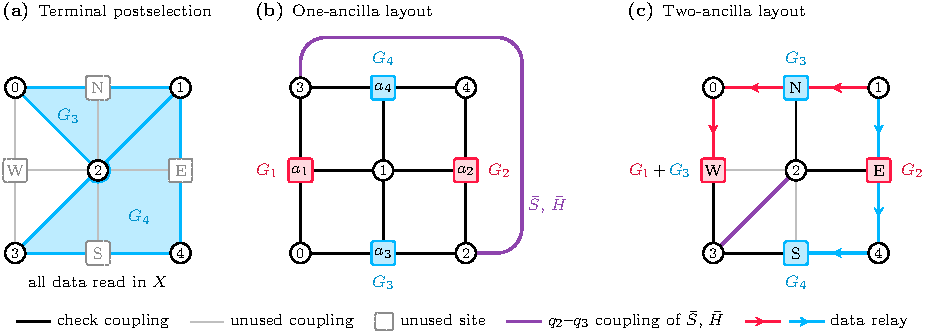
\includegraphics{figures/ancilla-layouts.pdf}% drawn at final size
  \caption{Stabilizer checks of the $[[5,1,2]]_3$ code on the conventional surface-code grid of data qutrits (circles) and ancilla sites (squares). Black and arrowed lines are couplings used by the check rounds; gray lines and dashed squares are unused. Red marks the $Z$-type $G_1$, $G_2$ and blue the $X$-type $G_3$, $G_4$. Purple lines mark the $q_2$--$q_3$ coupling of $CZ_{2\to3}$ in $\bar S$ and $\mathrm{SWAP}_{2,3}$ in $\bar H$. The label beside a site is its one readout per check round, modulo three and up to the syndromes' signs.
(a)~On the patch of \autoref{fig: 5-qutrit-code}, with $q_2$ at the center, terminal postselection uses no ancillas. The final $X$-basis readout of all data, with outcomes $x_j$, gives $G_3$, $G_4$ (shaded) and the logical outcome $x_0 + x_3$, not $G_1$ or $G_2$.
(b)~With $q_1$ at the center, ancilla $a_j$ neighbors all three data qutrits of $G_j$, but $q_2$ and $q_3$ sit at opposite corners and need a long-range coupling.
(c)~With $q_2$ at the center, $q_2$ and $q_3$ are diagonal neighbors, but $G_1$ and $G_4$ contain the opposite corners $q_1$ and $q_3$ and need two sites each. Arrows trace the data relay of their $q_1$ parts (\autoref{tab:conv_round}). N, holding $G_3$, collects the $q_1$ part of $G_1$ and lends its value to $q_0$, where W collects it with the rest of $G_1$, so W reads $G_1$ shifted by $G_3$. N then takes the value back and clears its $q_1$ part. E relays the $q_1$ part of $G_4$ likewise, through $q_4$ to S in the $X$ basis, before measuring $G_2$. All four readouts vanish exactly when all four syndromes do.}
  \label{fig:ancilla_layouts}
\end{figure}


\paragraph{One-ancilla layout.} This layout places $q_1$ at the center, with $q_3$, $q_4$, $q_0$ and $q_2$ at the top-left, top-right, bottom-left and bottom-right corners (\autoref{fig:ancilla_layouts}(b)). Every stabilizer contains $q_1$ and two adjacent corners, so each has one site next to its three data qutrits: $G_4$ is measured at the top site, $G_1$ at the left, $G_2$ at the right and $G_3$ at the bottom. Each stabilizer $G_j$ has its own ancilla $a_j$ on its site, for $9$ qutrits in total, and the check round uses all 12 site--data couplings of the grid. For the $Z$-type stabilizers $G_1$ and $G_2$, the three data qutrits control SUM or inverse SUM gates onto the ancilla (\autoref{fig:lrb_c}). For the $X$-type stabilizers $G_3$ and $G_4$, the ancilla is rotated by $H_3$, controls SUM or inverse SUM gates onto the data qutrits, and is rotated back by $H_3^{-1}$ before its computational-basis readout (\autoref{fig:lrb_d}). The two-qutrit gates of the logical $\bar H$ and $\bar S$, $\mathrm{SWAP}_{2,3}$ and $CZ_{2\rightarrow 3}$ (\autoref{eq:logical_HS}), act on $q_2$ and $q_3$, which in this layout sit at opposite corners, so the layout needs one long-range coupling, between $q_2$ and $q_3$. A check round occupies $9$ moments: one reset moment, $7$ gate moments with $12$ two-qutrit gates, and one readout moment.

\paragraph{Two-ancilla layout.} This layout places $q_2$ at the center, as in \autoref{fig: 5-qutrit-code}, with $q_0$, $q_1$, $q_3$ and $q_4$ at the top-left, top-right, bottom-left and bottom-right corners (\autoref{fig:ancilla_layouts}(c)). We call the sites N, W, E and S. N is next to $q_0$, $q_1$ and $q_2$, W to $q_0$, $q_2$ and $q_3$, E to $q_1$, $q_2$ and $q_4$, and S to $q_2$, $q_3$ and $q_4$. In this layout $q_2$ and $q_3$, on which the two-qutrit gates of $\bar H$ and $\bar S$ act, are diagonal neighbors. N measures $G_3$ and E measures $G_2$. $G_1$ and $G_4$, the boundary stabilizers, bypass $q_2$ (\autoref{fig: 5-qutrit-code}(d)) and both contain the opposite corners $q_1$ and $q_3$, so no site is next to all three of their data qutrits. Other generating sets do not avoid this, since the other elements of the stabilizer group that could replace $G_1$ or $G_4$ have weight four or five. Each boundary stabilizer therefore needs two sites, N and W for $G_1$ and E and S for $G_4$, which gives the layout its name. Reading the two parts of a boundary stabilizer on separate sites and adding the outcomes does not measure it, because reading a site measures the operator that the site has collected on the data. If N collects $Z_0 Z_1^{-1}$ and E collects $X_1^{-1} X_4^{-1}$, for example, then W reads $Z_3^{-1}$ and S reads $X_3$, so every round measures $q_3$ in the $Z$ and in the $X$ basis, and each readout randomizes the other.

We therefore pass the partial value through a data qutrit, a scheme we call a data relay, so that a single site holds the whole stabilizer before any site is read (\autoref{tab:conv_round}). Write $z_j$ for the computational-basis value of $q_j$, so that the syndrome of $G_1$ is $z_0 - z_1 - z_3$ modulo three. N first measures $G_3$. It then collects $-z_1$ and lends its value to $q_0$ with a SUM gate, which adds it to the value of $q_0$. W collects this value and $-z_3$. N then takes its value back from $q_0$ and clears its $-z_1$ part against $q_1$. Because N still holds its $G_3$ value while it lends, W reads the syndrome of $G_1$ shifted by the value of N. $G_4$ is measured in the same way in the $X$ basis: E collects its $q_1$ part and lends it to $q_4$, S collects $q_4$ and $q_3$, and E takes the value back before it measures $G_2$. Every site is read once per round. N reads the syndrome of $G_3$, W that of $G_1$ shifted by the value of N, E that of $G_2$ and S that of $G_4$, each up to its sign convention. A round passes when all four readouts are $0$, which is the case exactly when all four syndromes vanish. With a single fault in an otherwise noiseless round, no one-qutrit Pauli fault at any location and no two-qutrit Pauli fault after any two-qutrit gate leads to a logical error that this round and the next both miss, as in the one-ancilla round.

A check round occupies $13$ moments: one reset moment, $11$ gate moments with $18$ two-qutrit gates and six one-qutrit gates, and one readout moment (\autoref{tab:conv_round}). It uses 10 of the 12 site--data couplings of the grid, since W and S never act on $q_2$. Compared with the one-ancilla round, it adds six two-qutrit gates, two one-qutrit gates and four gate moments, and it resets and reads out the same number of ancillas. In both layouts every two-qutrit gate of a check round acts on a data qutrit. The one-ancilla layout leads our results, and \autoref{sub:layout_comparison} compares the two layouts.

% Moments as scheduled by the production generator: FoldedQutritConventionalSitesDetectionCode.conventional_sites_check_round_circuit (conventional-sites worktree, src/lrb/code_definitions.py), rescheduled with LRBCircuitGenerator.schedule_moments in paper-rework/scratch/writer-conv/budget.py (budget.out)
\begin{table}[htb]
  \centering
  \small
  \begin{tabular}{c|l}
    \hline
    moment & gates \\
    \hline
    1 & $H_3$ on E, S and N \\
    2 & $\mathrm{SUM}(\mathrm{E} \to q_1)$, $\mathrm{SUM}^{-1}(\mathrm{S} \to q_3)$, $\mathrm{SUM}(\mathrm{N} \to q_0)$ \\
    3 & $\mathrm{SUM}(q_4 \to \mathrm{E})$, $\mathrm{SUM}^{-1}(q_3 \to \mathrm{W})$, $\mathrm{SUM}^{-1}(\mathrm{N} \to q_2)$ \\
    4 & $\mathrm{SUM}(\mathrm{S} \to q_4)$, $\mathrm{SUM}(\mathrm{N} \to q_1)$ \\
    5 & $H_3^{-1}$ on S, $\mathrm{SUM}^{-1}(q_4 \to \mathrm{E})$, $H_3^{-1}$ on N \\
    6 & $\mathrm{SUM}^{-1}(\mathrm{E} \to q_1)$ \\
    7 & $\mathrm{SUM}^{-1}(q_1 \to \mathrm{N})$, $H_3^{-1}$ on E \\
    8 & $\mathrm{SUM}(\mathrm{N} \to q_0)$, $\mathrm{SUM}(q_2 \to \mathrm{E})$ \\
    9 & $\mathrm{SUM}^{-1}(q_4 \to \mathrm{E})$, $\mathrm{SUM}(q_0 \to \mathrm{W})$ \\
    10 & $\mathrm{SUM}^{-1}(\mathrm{N} \to q_0)$, $\mathrm{SUM}(q_1 \to \mathrm{E})$ \\
    11 & $\mathrm{SUM}(q_1 \to \mathrm{N})$ \\
    \hline
  \end{tabular}
  \caption{Gate moments of one check round in the two-ancilla layout, as scheduled in the simulations. $\mathrm{SUM}(a \to b)$ adds the computational-basis value of $a$ to $b$, and $\mathrm{SUM}^{-1}(a \to b)$ subtracts it. For a site in the $X$ basis, between $H_3$ and $H_3^{-1}$, $\mathrm{SUM}(a \to b)$ instead subtracts the $X$-basis value of $b$ from that of $a$, so $X$-basis values move against the arrow. N, W, E and S are the sites of \autoref{fig:ancilla_layouts}(c). The round starts with one reset moment of the four sites and ends with one readout moment of the four sites. In moments 1 to 5, N measures $G_3$ and S measures $G_4$, while E collects its $q_1$ part, lends it to $q_4$ in moment 3 and takes it back in moment 5. In moments 6 and 7, E clears itself against $q_1$ and N collects $-z_1$. W collects $-z_3$ in moment 3 and, in moment 9, all of $q_0$, which then holds $z_0$ plus the lent value, between the lend of N in moment 8 and its return in moment 10, and N clears itself against $q_1$ in moment 11. E measures $G_2$ in moments 8 to 10.}
  \label{tab:conv_round}
\end{table}

\subsubsection{Physical RB Baseline}
\label{sub:rb_baseline}

We compare every LRB-D configuration with single-qutrit physical RB simulated under the same noise model at the same value of $p$. The baseline uses the mirror construction of LRB-D on one qutrit, in the spirit of mirror randomized benchmarking~\cite{Proctor2022MirrorRB}, rather than a single recovery gate $C_{\text{inv}} = (C_m \cdots C_1)^{-1}$. We prepare $\ket{0}$, apply Cliffords $C_1, \dots, C_m$ drawn uniformly from the same $216$-element catalog, apply the mirror inverse $C_m^{-1}, \dots, C_1^{-1}$, and measure in the computational basis. A circuit of depth $m$ again contains $2m$ noisy Cliffords. Each Clifford is a word in the primitive gates $H$, $S$, $X$ and $Z$ (\autoref{sec:clifford-gen}). Every primitive gate, including the Pauli gates and the identity, is applied as a separate gate followed by DEP1, with probability $p/10$ under SI1000 and $p$ under SD6. The final measurement is noiseless. As for LRB-D, we record the modulus of $P_0 + P_1\omega + P_2\omega^2$ for each sequence and average it over the sequences. We sample $10^4$ shots per sequence and depth, with the same depths and the same number of random sequences as LRB-D (\autoref{sub:results_setup}). The RB sequences are drawn independently of the LRB-D sequences, every run draws its own, and every shot is kept.

The single-qutrit circuit contains no two-qutrit gates, resets, mid-circuit measurements or idle qutrits, so the baseline experiences only the one-qutrit gate channel. Under SI1000 that channel has probability $p/10$, ten times below the probability $p$ of the two-qutrit gates in every check round and in the logical $\bar H$ and $\bar S$ of the encoded circuits. LRB-D under SI1000 is therefore compared with a physical qutrit whose gates are ten times better than the entangling gates of the code. Under SD6 every operation fails with probability $p$, and the baseline is a physical qutrit whose gates fail as often as every operation in the encoded circuit.

\subsubsection{Fit Model and Error Rates}
\label{sub:fit_model}

% Finite-shot floor of the modulus (about 0.886/sqrt(N) for N shots with uniformly random outcomes) and the SD6 RB data at large depth: paper-rework/scratch/physics-reviewer-e2/rbfloor.py (.out)
For each postselection schedule and each value of $p$, we fit the sequence-averaged $|\langle \bar{X} \rangle|$ as a function of the depth $m$ to Eq.~\eqref{eq:fseq} with $B = 0$,
\begin{equation}
    F(m) = A f^{m},
    \label{eq:zero_offset_fit}
\end{equation}
by weighted least squares, weighting each depth by the inverse variance of $|\langle \bar{X} \rangle|$ over the random sequences. We fit the physical RB baseline with the same model. We fix $B = 0$ because our observable is the modulus of a generalized Pauli expectation value, not a survival probability. A fully depolarized qutrit gives $(1 + \omega + \omega^2)/3 = 0$, so the decay has no constant offset. Fixing $B$ also removes the near-degeneracy between $A$ and $B$ when $f$ is close to one over the available depths. SPAM errors then enter only through $A$. The zero offset holds for the expectation value but not for its finite-shot estimate, whose modulus has a positive floor: for $N$ shots with uniformly random outcomes it averages about $0.9/\sqrt{N}$. The floor matters for points with few accepted shots (\autoref{sub:interval_results}) and for the SD6 RB data, with $10^4$ shots per sequence, at the largest depths for $p \ge 0.02$, which approach or level off at about $0.009$. The SI1000 RB data stay far above the floor. The LRB-D fit uses every depth, $m = 0$ included, at which every random sequence keeps at least one shot, except that the fits of the high-$p$ extension runs for $k \ge 2$ use only their even depths $m = 0, 2, 4$ and $6$ (\autoref{sub:results_setup}). At large $p$ almost no shot survives at large depth, and the fits use fewer depths, as few as two.

The decay parameter $f$ gives the average fidelity through Eq.~\eqref{eq:fbar} with $q = 3$,
\begin{equation}
    \bar{F} = \frac{2f + 1}{3}, \qquad r = 1 - \bar{F} = \frac{2}{3}\,(1 - f) .
    \label{eq:error_rate}
\end{equation}
One unit of depth adds one forward Clifford and its mirror inverse, and in LRB-D also one check round. The fitted $f$, $\bar{F}$ and $r$ are therefore per unit of depth, that is, per forward logical Clifford plus its mirror inverse. We report every fidelity and error rate in this convention, including those in the figure legends. A per-Clifford decay parameter would be $f^{1/2}$, with an error rate close to $r/2$ when $r$ is small.

We define the pseudo-threshold $p^\star(k)$ as the value of $p$ at which the LRB-D error rate with interval $k$ equals the physical RB error rate at the same $p$ (\autoref{sub:pseudo_thresholds}). Both error rates are per unit of depth, and $r$ decreases monotonically with $f$. The condition $r_{\mathrm{LRB}} = r_{\mathrm{RB}}$ is therefore equivalent to $f_{\mathrm{LRB}} = f_{\mathrm{RB}}$ and to $f_{\mathrm{LRB}}^{1/2} = f_{\mathrm{RB}}^{1/2}$, so the pseudo-thresholds do not depend on the depth convention.

We estimate error-rate uncertainties with a parametric bootstrap. We perturb every sequence-averaged point by Gaussian noise whose width is its standard error over the random sequences, refit, repeat this $500$ times, and quote the standard deviation and the central $68\%$ interval of the refitted error rates.
Each perturbed point is clipped to $[0, 1]$ before the refit. The LRB-D and RB refits both use the zero-offset model of Eq.~\eqref{eq:zero_offset_fit}, the same model as the point estimates. The bootstrap perturbs every depth independently. All depths of a sequence share its first Cliffords, so a different draw of sequences shifts all depths together, and this bootstrap does not include the uncertainty from the choice of sequences (\autoref{sub:results_setup}). Its standard deviations accompany the LRB-D error rates of \autoref{tab:k1_error_rates} and the comparisons of fitted error rates in \autoref{sub:results_setup}, and its $68\%$ intervals are the error bars on the fitted error rates in the figures.

% Sequence bootstrap of the pseudo-thresholds: scripts/sequence_bootstrap_thresholds.py, outputs in LRB-experiment-data-slurm/comparisons/sequence-bootstrap/ (seq_boot_se copied to comparisons/pseudo-thresholds-current.csv); seq_boot_valid_fraction = 1.0 for all 16 entries; paired interval gaps in sequence-bootstrap/interval_gap_significance.csv, checked by paper-rework/scratch/writer-seq-se/paired.py (paired.out)
For the pseudo-thresholds, uncertainties are one standard error (68\% confidence), from a bootstrap over the random Clifford sequences. One sequence draw is shared by every depth and every $p$, so the correlations that come from reusing the same sequences are included. The bootstrap has $1000$ replicates. Each replicate draws 30 sequences with replacement from the 30 random sequences of a run and applies this draw to every depth and every $p$ of that sequence set. The sequence sets of the production LRB-D runs, the extension LRB-D runs, the production RB and the extension RB are resampled independently. From the outcome counts of the drawn sequences we rebuild the sequence averages and their spread over the sequences at every depth, refit every LRB-D and RB curve with the zero-offset model of Eq.~\eqref{eq:zero_offset_fit} and the depth rule of the point estimates, $m = 0$ included, and recompute $p^\star(k)$ with the crossing rule of \autoref{sub:pseudo_thresholds}. The standard error is the standard deviation of $p^\star(k)$ over the replicates, that is, the error of the mean over the ensemble of random sequences. Every replicate finds a crossing. The per-sequence RB outcomes were not stored. We therefore re-simulate the RB sequences once with the production settings, $10^4$ shots per sequence and depth, and in each replicate shift the fitted RB error rate of the run by the change that the resampling produces in the fit to the re-simulated data. Differences between pseudo-thresholds of one configuration are evaluated replicate by replicate, so that the shared sequences enter both values. Different configurations come from independent runs with their own sequences, so when two of their pseudo-thresholds are compared through their ratio, the relative standard errors add in quadrature (\autoref{sub:pseudo_thresholds}).

\subsubsection{Irreducible Representations and Syndrome Dynamics}
\label{sub:irreps}

The behavior of the twirled error channel in the logical setting can be explained by studying the representation theory of the Clifford group.
A short review of the relevant representation theory is included in \Cref{sec:rep-theory}.

The logical Clifford group $\bar{\mathcal{C}}_3$ defines a representation of the single-qutrit Clifford group $\mathcal{C}_3$.
Importantly, the module corresponding to this representation is not the $3^5$ dimensional physical space $\mathcal{H}_{phys}$, but instead the $9^5$ dimensional space $\mathcal{B}({\mathcal{H}_{phys}})$.
To avoid confusion, we will denote by $\mathcal{S}_{phys}$ the space of linear maps $\mathcal{B}(\mathcal{H}_{phys})$.
The representation $\bar{\pi} : \mathcal{C}_3 \to 
\mathrm{End}(\mathcal{S}_{phys})$ defined by the logical Clifford group is the typical conjugation
$$
\bar{\pi}(C)(\rho) = \bar{C} \rho \bar{C}^\dagger,
$$
where $\bar{C}$ is the five-qutrit unitary that implements $C$ on the logical qutrit, taken from the group generated by the physical $\bar H$ and $\bar S$ of Eq.~\eqref{eq:logical_HS}. Up to global phases this group has $216$ elements and maps one-to-one onto $\mathcal{C}_3$, so $\bar{\pi}$ is a representation of $\mathcal{C}_3$.
By Maschke's theorem, $\mathcal{S}_{phys}$ decomposes as a direct sum of irreducible representations (irreps).
The Clifford group has $10$ irreps, one for each conjugacy class \ACE{cite the paper that lists conjugacy classes}, but only two of them are important to us. Up to global phases its $10$ conjugacy classes have sizes $1, 8, 9, 12, 12, 24, 24, 36, 36$ and $54$, and its irreps have dimensions $1, 1, 1, 2, 2, 2, 3, 8, 8$ and $8$.
The first is the trivial irrep $V_{triv}$ and the second is the eight dimensional irrep $V_{pauli}$ coming from conjugation of the $8$ traceless Pauli matrices.
The remaining irreps will be denoted as $V_i$ for $i \geq 2$. In this notation, we obtain the decomposition
\begin{align}
    \mathcal{S}_{phys} \cong m_{triv} V_{triv} \oplus m_{pauli} V_{pauli} \oplus \bigoplus_{i = 2}^{9} m_i V_i
\end{align}
where the $m_i$ denote the multiplicity of each irrep in the direct sum.
% Verified 2026-10-31 (paper-rework/scratch/lead/irreps_check.py): conjugation representation of the 216-element group generated by the physical Hbar and Sbar built with sdim's gate matrices; Burnside character table of the logical action; multiplicities 301, 260, 260 (dim 1), 560, 560, 520 (dim 2), 820 (dim 3), 2160, 2160, 2241 (dim 8, the last being V_pauli), sum m*d = 59049. The earlier hand value m_triv = 201 (total 2442) was a slip.
Using the orthogonality of characters, we can compute $m_{triv} = 301$ and $m_{pauli} = 2241$. The other multiplicities are $260$ and $260$ for the remaining one-dimensional irreps, $560$, $560$ and $520$ for the two-dimensional ones, $820$ for the three-dimensional one, and $2160$ and $2160$ for the other two eight-dimensional ones, so that $\sum_i m_i \dim V_i = 3^{10}$. The simulated Clifford catalog applies the logical Paulis as the physical $\bar X$ and $\bar Z$ of \autoref{eq:logicalPauli}, which differ from their images in the group generated by $\bar H$ and $\bar S$ by the stabilizers $G_4$ and $G_2$. With them the generated group has $1944$ elements, $m_{triv} = 40$ and $m_{pauli} = 261$, while its action on the code space is unchanged.
Noting that in the one-qutrit case $m_{triv} = m_{pauli} = 1$ and every other multiplicity is $0$, we can already see a stark difference between the five- and one-qutrit cases.

Let $\mathrm{End}_{\bar{\mathcal{C}}_3}(\mathcal{S}_{phys})$ denote the subset of linear maps $T : \mathcal{S}_{phys} \to \mathcal{S}_{phys}$ that commute with the action of $\mathcal{C}_3$.
A corollary of Schur's lemma tells us that $\mathrm{End}_{\bar{\mathcal{C}}_3}(\mathcal{S}_{phys})$ is isomorphic, as an algebra, to a direct sum of matrix algebras as in
\begin{align}
    \mathrm{End}_{\bar{\mathcal{C}}_3}(\mathcal{S}_{phys}) &\cong \mathrm{Mat}_{m_{triv}}(\mathbb{C}) \otimes I_{V_{triv}} \oplus \mathrm{Mat}_{m_{pauli}}(\mathbb{C})\otimes I_{V_{pauli}} \oplus \bigoplus_{i = 2}^9 \mathrm{Mat}_{m_i} (\mathbb{C}) \otimes I_{V_i}\\
    &\cong \mathrm{Mat}_{m_{triv}}(\mathbb{C}) \oplus \mathrm{Mat}_{m_{pauli}}(\mathbb{C}) \oplus \bigoplus_{i = 2}^9 \mathrm{Mat}_{m_i}(\mathbb{C}) .
\end{align}
This corresponds to the fact that a $\mathcal{C}_3$-linear endomorphism cannot map a vector in $m_i V_i$ to a vector whose support intersects nontrivially with $m_j V_j$ when $i \neq j$.
Notice that the twirled error channel is constructed to be $\mathcal{C}_3$-linear and thus admits such a decomposition
\begin{align}
    \Lambda_{eff} = M_{triv}\otimes I_{V_{triv}} \oplus M_{pauli} \otimes I_{V_{pauli}} \oplus M
\end{align}
in an appropriate basis.
If $M_{triv}$ and $M_{pauli}$ are diagonalizable, then up to another change of basis we may write the effective error channel
\begin{align}
    \Lambda_{eff} = \Lambda_{triv} \oplus \Lambda_{pauli} \otimes I_{V_{pauli}} \oplus M
\end{align}
where $\Lambda_{triv}$ and $\Lambda_{pauli}$ are the diagonal matrices of eigenvalues for $M_{triv}$ and $M_{pauli}$ respectively.
The final $M$ denotes the total contribution for all $8$ other irreps.
As long as our initial state lies in the code space, as the logical stabilizer state $\ket{\bar{+}}$ does, the matrix $M$ is entirely inconsequential.
This follows as such a state $\rho$ will have decomposition
\begin{align}
    \rho = \rho_{triv} \oplus \rho_{pauli} \oplus 0
\end{align}
for $\rho_{triv} \in m_{triv} V_{triv}$ and $\rho_{pauli} \in m_{pauli}V_{pauli}$.
Thus the dynamics of the effective channel are succinctly described by the $m_{triv} + m_{pauli} = 301 + 2241 = 2542$ diagonal elements of $\Lambda_{triv}$ and $\Lambda_{pauli}$.
While this is a much smaller number than $9^5$, it is much larger than the $1 + 1 = 2$ relevant eigenvalues in the one-qutrit case.

With $\Lambda_{eff}$ diagonalized, it is quite simple to see what repeated application of the error channel will look like. Namely, we have the identity 
\begin{align}
    \Lambda_{eff}^n = \Lambda_{triv}^n \oplus \Lambda_{pauli}^n \otimes I_{V_{pauli}} \oplus M^n.
\end{align}
If $M_{triv}$ or $M_{pauli}$ is not diagonalizable, we use its Jordan form instead. A Jordan block of size $s$ with eigenvalue $\lambda$ then contributes terms $\binom{n}{j}\lambda^{n-j}$ with $j < s$ in place of the single power $\lambda^n$.

%%% REP THEORY MOVED TO "rep theory appendix.tex" AIDAN 1/19/26



\subsection{Noise Models}
\label{sub:noise_models}

We simulate LRB-D under two circuit-level noise models of Gidney, Newman, Fowler and Broughton \cite{GidneyHoneycomb2021}, which we generalize to qutrits. SD6 is a uniform depolarizing model in which every operation fails with the same probability. SI1000 (superconducting-inspired) assigns different rates to different operations. Both models have a single parameter $p$, the depolarizing probability of a two-qutrit gate, and every other rate is a fixed multiple of $p$. We sweep $p$, and all error rates in \autoref{sec:results} are plotted against $p$. Both models are built entirely out of qutrit Pauli channels. This keeps every noisy circuit inside the stabilizer formalism and permits the sampling methods of \autoref{sub:sim_framework}.

\subsubsection{Qutrit Pauli Channels}

\texttt{sdim} implements the depolarizing channel of Eq.~\eqref{eq:1-depol} in its Weyl form: with probability $p$ it applies a uniformly random non-identity Pauli $X^a Z^b$ to the qutrit,
\begin{equation}
    \mathcal{E}_{\mathcal{D}}(p)(\rho) = (1-p)\,\rho + \frac{p}{8}\sum_{P \neq I} P \rho\, P^\dagger .
\end{equation}
The two conventions describe the same family of channels and are related by $p_{\mathrm{mix}} = \tfrac{9}{8}\,p$, because one ninth of the uniform Pauli mixture reproduces the input state. The two-qutrit channel is defined the same way,
\begin{equation}
    \mathcal{E}^{(2)}_{\mathcal{D}}(p)(\rho) = (1-p)\,\rho + \frac{p}{80}\sum_{P \neq I \otimes I} P \rho\, P^\dagger,
    \label{eq:2-depol}
\end{equation}
with $P$ ranging over the $80$ non-identity two-qutrit Paulis, and corresponds to the mixing form $(1-p_{\mathrm{mix}})\,\rho + \tfrac{p_{\mathrm{mix}}}{9} I$ with $p_{\mathrm{mix}} = \tfrac{81}{80}\,p$. Following \cite{GidneyHoneycomb2021}, we call $\mathcal{E}_{\mathcal{D}}$ and $\mathcal{E}^{(2)}_{\mathcal{D}}$ DEP1 and DEP2. The classical bit flips that the qubit models attach to resets and measurements become uniform shift channels,
\begin{equation}
    \mathcal{F}_X(x)(\rho) = (1-x)\,\rho + \frac{x}{2}\left( X \rho X^\dagger + X^2 \rho\, (X^2)^\dagger \right),
    \label{eq:flip-channel}
\end{equation}
together with the phase channel $\mathcal{F}_Z(x)$, in which $Z$ and $Z^2$ replace $X$ and $X^2$. A shift $X^a$ with $a \neq 0$ immediately before a computational-basis measurement $M$ changes the recorded outcome by $a$ modulo three. A phase $Z^a$ plays the same role before an $X$-basis measurement $M_X$. In everything that follows, $p$ and every rate derived from it are Weyl-form probabilities, that is, the probability that the simulator applies a non-identity error.

\subsubsection{Moments, Segments and Noise Placement}

We divide every circuit into segments. Each logical Clifford, each stabilizer check round and each physical Clifford of the RB baseline is its own segment. Within a segment, gates are scheduled as soon as possible into moments: every operation goes into the earliest moment after the previous operation on each of its qutrits. Operations on disjoint qutrits therefore run in parallel, and the order on each qutrit is kept. A moment holds either unitary gates or collapse operations (resets and measurements), never both. Measurements whose qutrit is not used again in the segment are moved to one final moment, so all ancilla readouts of a check round share its last moment. Moments never span two segments.

Every moment then receives noise according to \autoref{tab:circuit-noise}. DEP1 follows every one-qutrit gate and DEP2 follows every two-qutrit gate. $\mathcal{F}_X$ follows every reset. A flip precedes every measurement, $\mathcal{F}_X$ before $M$ and $\mathcal{F}_Z$ before $M_X$, and DEP1 follows it. Every qutrit that a moment leaves untouched receives idle DEP1, at one rate in gate moments and at another in measurement and reset moments. An explicit identity gate occupies a moment and receives the idle noise of a gate moment.

\begin{table}[H]
  \centering
  \begin{tabular}{l|c|c|c}
    \hline
    Circuit location & Channel & SI1000 & SD6 \\
    \hline
    After each one-qutrit gate & $\mathcal{E}_{\mathcal{D}}$ & $p/10$ & $p$ \\
    After each two-qutrit gate & $\mathcal{E}^{(2)}_{\mathcal{D}}$ & $p$ & $p$ \\
    After each reset & $\mathcal{F}_X$ & $2p$ & $p$ \\
    Before each computational-basis measurement $M$ & $\mathcal{F}_X$ & $5p$ & $p$ \\
    Before each $X$-basis measurement $M_X$ & $\mathcal{F}_Z$ & $5p$ & $p$ \\
    After each measurement & $\mathcal{E}_{\mathcal{D}}$ & $p$ & $p$ \\
    Idle qutrit in a gate moment & $\mathcal{E}_{\mathcal{D}}$ & $p/10$ & $p$ \\
    Idle qutrit in a measurement or reset moment & $\mathcal{E}_{\mathcal{D}}$ & $2p$ & $p$ \\
    \hline
  \end{tabular}
  \caption{Qutrit SI1000 and SD6 noise models. Each entry is the probability of the channel in the second column, as a function of the swept parameter $p$, the two-qutrit gate depolarizing probability. SI1000 requires $p \le 0.2$ so that the measurement flip probability $5p$ is at most one.}
  \label{tab:circuit-noise}
\end{table}

SD6 treats every operation as equally noisy. SI1000 encodes the hierarchy of superconducting processors described in \cite{GidneyHoneycomb2021}. One-qutrit gates and qutrits idling in gate moments fail with probability $p/10$. Measurement results flip with probability $5p$ and resets with probability $2p$. Qutrits that idle while other qutrits are measured or reset depolarize with probability $2p$. Two features of our circuits limit which rules act. All ancilla readouts are computational-basis measurements, because the $X$-type checks rotate their ancillas with $H^{-1}$ before $M$, so the $\mathcal{F}_Z$ rule never applies. Post-measurement DEP1 acts only on ancillas that are reset before their next use or never used again, so it affects no detector and no logical observable.

% TODO(authors): confirm that these deviations from the reference noise models are intended (native SUM, CZ and SWAP under both models, no stacking of Idle(p/10) and ResonatorIdle(2p) under SI1000, post-measurement DEP1 in both models).
Our qutrit models differ from those of \cite{GidneyHoneycomb2021} in three respects. First, we add DEP1 after every measurement in both models. The reference models have no such rule, and in our circuits it has no effect, as explained above. Second, under SI1000 a qutrit that idles in a measurement or reset moment receives DEP1 with probability $2p$ only. In the reference, the rules Idle($p/10$) and ResonatorIdle($2p$) both act on such a qubit. Third, we treat SUM, CZ, their inverses and SWAP each as one native two-qutrit gate followed by DEP2. The reference gate sets contain a single entangling gate, CZ for SI1000 and CX for SD6, so there a SWAP, or an entangling gate of the other type, would be compiled into several entangling and one-qubit gates.

Three steps are noiseless in all simulations: the encoding of $\ket{\bar{+}}$ (\autoref{fig:encoding_circuit}), the terminal logical readout of LRB-D (\autoref{sub:lrb_d}), which includes the direct $X$-basis data readout of terminal postselection, and the final measurement of the physical RB baseline (\autoref{sub:rb_baseline}). The injected noise therefore acts only on the random Clifford sequence, its mirror inverse and the check rounds. On hardware these steps are noisy and contribute SPAM errors.

\subsection{Simulation Framework}
\label{sub:sim_framework}

All of our numerical results are produced with the \texttt{sdim} qudit stabilizer simulator \cite{sdim}, version 1.4.0, which extends tableau-based stabilizer simulation to prime-dimensional qudits and samples noisy circuits in the Pauli frame picture. \autoref{sec:sdim-dem} reviews the simulator in more detail. The circuits in this work are expressed in terms of the generalized Hadamard, phase, SUM and controlled-phase gates of \autoref{sec:bg}, the Pauli and SWAP gates, and their inverses, computational-basis measurements, ancilla resets, and the one- and two-qutrit Pauli noise channels of \autoref{sub:noise_models}.

For each random sequence we draw the Cliffords for the largest depth once and build every depth from them: depth $m$ uses $\bar C_1, \dots, \bar C_m$ and the inverses $\bar C_m^{-1}, \dots, \bar C_1^{-1}$. For each sequence and depth we generate one annotated \texttt{sdim} circuit with check rounds, which serves every uniform-interval schedule, and one check-free circuit with the same Cliffords for terminal postselection. The physical RB circuits use their own random sequences. Each circuit contains the scheduled logical gates and check rounds, the noise operations of \autoref{sub:noise_models}, and \texttt{DETECTOR} and \texttt{LOGICAL\_OBSERVABLE} declarations. A detector is a linear combination of measurement outcomes that is deterministic in the absence of noise. Here each detector is one ancilla readout of one check round, or in terminal postselection one classically evaluated $X$-type stabilizer. The logical observable is the terminal readout of $\bar X$. Each noise operation stores its probability as a multiple of $p$ (\autoref{tab:circuit-noise}). For every value of $p$ we set each probability to that multiple of $p$, so one generated circuit structure per sequence and depth serves the entire sweep. The Clifford catalog is built with the Cayley graph construction of \autoref{sec:clifford-gen}, and the inverse of each element reverses its word and inverts every symbol, without resynthesis. The mirror inverse applies the looked-up inverse of each sampled Clifford, one Clifford at a time in reverse order, rather than a single recovery gate.

The annotated circuits can be sampled with two backends. The first is direct Pauli-frame simulation. The second compiles each circuit into a compact $q$-ary detector error model (DEM), a structure introduced for qubit stabilizer circuits by the Stim simulator \cite{Gidney2021Stim}. We use the native DEM of \texttt{sdim} 1.4.0, \texttt{sdim.dem.DetectorErrorModel}, which turns each noise operation that a detector or the logical observable can see into one error mechanism and represents the depolarizing and shift channels exactly. Postselected LRB-D statistics can then be sampled at a cost that no longer depends on the size of the underlying stabilizer computation. All four production runs, the one- and two-ancilla layouts under SI1000 and SD6, use the DEM backend for the LRB-D, terminal postselection and physical RB circuits, and so do the four high-$p$ extension runs, one per layout and noise model (\autoref{sub:results_setup}). %
% DEM versus frame sampler for the two-ancilla (conventional-site) code: paper-rework/scratch/writer-conv/demcheck/run_check.py (run_check.out); one-ancilla code: tests/test_dem_backend.py
On depth-$2$ circuits of both layouts under both models at $p = 0.01$, the per-round pass rates and logical outcomes from the two backends agree within five standard errors over $4 \times 10^4$ shots. \autoref{sec:sdim-dem} explains the construction, why it is exact for our noise models, and how it is sampled.


\subsection{Qubit \texorpdfstring{$[[5,1,2]]$}{[[5,1,2]]} Code}
\label{sub:qubit_code}

% Qubit code and catalog: FoldedQubitDetectionCode and QubitCliffordLibrary (worktree qubit-lrbd-sdim140, src/lrb/code_definitions.py), FoldedQubitConventionalSitesDetectionCode (worktree conventional-sites); checks in tests/test_folded_qubit_code.py and tests/test_conventional_sites_code.py of those worktrees. Word lengths, run settings, threshold-rule checks and brackets: paper-rework/scratch/writer-qubit/analysis.py (analysis.out, sections A, A2, X5, T1, T2, X1, B1)
To separate the role of the local dimension, we repeat the simulations of \autoref{sec:results} for the qubit version of the code, with local dimension $q = 2$ in place of $q = 3$ (\autoref{sub:qubit_comparison}). The qubit $[[5,1,2]]$ code has the stabilizers of Eqs.~\eqref{eq:s1}--\eqref{eq:s4} with every exponent taken modulo two,
\begin{equation}
  G_1 = Z_0 Z_1 Z_3, \qquad G_2 = Z_1 Z_2 Z_4, \qquad G_3 = X_0 X_1 X_2, \qquad G_4 = X_1 X_3 X_4,
\end{equation}
and the logical operators $\bar X = X_0 X_3$ and $\bar Z = Z_0 Z_2$ of Eq.~\eqref{eq:logicalPauli}. The transversal gates of Eq.~\eqref{eq:logical_HS} keep their form, with the qubit phase gate $S = \mathrm{diag}(1, i)$ and $H^\dagger = H$. $\bar H$ applies $\mathrm{SWAP}_{2,3}$ and then $H$ to $q_0$, $q_2$, $q_3$ and $q_4$ and $H^\dagger$ to $q_1$, and $\bar S$ applies $S$ to $q_0$ and $q_4$, $S^\dagger$ to $q_1$ and $CZ$ to $q_2$ and $q_3$. The logical Cliffords are drawn uniformly from the full $24$-element single-qubit Clifford group, whose elements we write as the products of the Paulis $I$, $X$, $Z$ and $XZ$ with the six words $I$, $H$, $S$, $HS$, $SH$ and $HSH$, with identity factors dropped as in \autoref{sec:clifford-gen}. These strings contain between one and five symbols, $61/24 = 2.54$ on average, against $5.17$ for the $216$ qutrit strings. As for qutrits, each inverse reverses its word and inverts every symbol. The encoded circuits of all $24$ Cliffords and of their inverses act on the code space as the intended single-qubit Cliffords, and in noiseless simulation of either layout every weight-one Pauli error on a data qubit gives a nontrivial syndrome in a check round.

% Qubit noise channels: sdim 1.4.0 (N1 'd' uniform over the q^2 - 1 non-identity Paulis, N1 'f'/'p' over the q - 1 nonzero shifts, N2 uniform over the q^4 - 1 non-identity Paulis) and CIRCUIT_LEVEL_NOISE_RATES in src/lrb/circuit_generator.py, identical in the qubit-lrbd-sdim140 and conventional-sites worktrees; mixing forms checked in paper-rework/scratch/corrector-qubit-1/corrector.py (section H)
The noise models apply the channels of \autoref{sub:noise_models} with $q = 2$, at the rates of \autoref{tab:circuit-noise}. DEP1 applies $X$, $Z$ or $XZ$ with probability $p/3$ each, which corresponds to $p_{\mathrm{mix}} = \tfrac{4}{3}\,p$, and DEP2 applies each of the $15$ non-identity two-qubit Paulis with probability $p/15$, which corresponds to $p_{\mathrm{mix}} = \tfrac{16}{15}\,p$. The flip channels $\mathcal{F}_X(x)$ and $\mathcal{F}_Z(x)$ apply $X$ or $Z$ with probability $x$, so that a flip before a measurement inverts the recorded bit. These are the DEP1, DEP2 and flip channels of \cite{GidneyHoneycomb2021}. The qubit SI1000 and SD6 models are therefore the reference models up to the three deviations of \autoref{sub:noise_models}: DEP1 after every measurement, idle DEP1 at $2p$ only in SI1000 measurement and reset moments, and CNOT, CZ and SWAP each as one native two-qubit gate followed by DEP2.

% Estimator floor for q = 2 (E|P0 - P1| about 0.80/sqrt(N) for uniformly random outcomes): paper-rework/scratch/corrector-qubit-1/corrector.py (section G)
Everything else is carried over unchanged: the nine wires, the encoding circuit of \autoref{fig:encoding_circuit}, the check rounds of both layouts, with CNOT in place of SUM, the depths, sequences and shots of \autoref{sub:results_setup}, the sampling through the detector error model of \texttt{sdim} (\autoref{sub:sim_framework}), the mirror inverse, and the fits of \autoref{sub:fit_model}, $m = 0$ included. With $\omega = -1$ the estimator $\sum_j \omega^{-j} P_j$ of \autoref{sub:lrb_d} becomes $\langle \bar X \rangle = P_0 - P_1$, and we again average its modulus over the sequences. A fully depolarized qubit gives $(1 - 1)/2 = 0$, so the zero offset $B = 0$ holds as for qutrits, and the finite-shot floor of the modulus is about $0.8/\sqrt{N}$ for $N$ shots. The physical baseline is single-qubit RB over the $24$ Cliffords, with $10^4$ shots per sequence and depth. Eq.~\eqref{eq:fbar} with $q = 2$ gives $\bar F = (f + 1)/2$ and $r = (1 - f)/2$, per unit of depth as before.

We locate the qubit pseudo-thresholds with the search of \autoref{sub:pseudo_thresholds} without its tolerance and error floor. The qubit $p^\star(k)$ is thus the value of $p$ at which the fitted LRB-D error reaches the RB error, interpolated linearly between the two bracketing grid points. On every qubit grid the difference between the two errors changes sign exactly once at $p > 0$, and the tail cut removes no point. The qutrit tolerance of $5\times10^{-4}$ and floor of $2\times10^{-3}$ are comparable to the qubit SI1000 error rates at the crossings, $1.0\times10^{-3}$ to $3.9\times10^{-3}$. With them the search would stop at a grid point below or above the crossing, and seven of the eight SI1000 values would move, by $-16.5$ to $+43.9\%$. Under SD6, where the error rates at the crossings are $1.6\times10^{-2}$ to $6.8\times10^{-2}$, they would move by at most $1.4\%$. On the qutrit grids the search without tolerance and floor returns all sixteen values of \autoref{tab:pseudo_thresholds} unchanged.

% Production-versus-refinement overlap (pipeline fits of both runs, parametric-bootstrap standard deviations added in quadrature): paper-rework/scratch/corrector-qubit-1/corrector.py (section E)
The qubit crossings lie at $p = 0.0031$ to $0.0112$ under SI1000 and $0.0047$ to $0.0210$ under SD6, below the high-$p$ extension ranges of \autoref{sub:results_setup}. Instead of a high-$p$ extension, the qubit pseudo-thresholds use one near-threshold refinement run per layout and noise model, with the production depths, $10^6$ LRB-D and $10^4$ RB shots per sequence and depth, and 30 newly drawn LRB-D and RB sequences on a finer grid of $p$. Under SI1000 this grid runs from $0.002$ to $0.013$ in steps of $0.0005$ in both layouts. Under SD6 it runs from $0.006$ to $0.026$ in steps of $0.001$ with one ancilla, and with two ancillas from $0.003$ to $0.0055$ in steps of $0.0005$ and from $0.006$ to $0.026$ in steps of $0.001$. Inside this window the refinement fits replace the production fits, for LRB-D and RB alike, and outside it the production fits are used. All refinement depths are even, as in the production grid. The pseudo-threshold uncertainties come from the sequence bootstrap of \autoref{sub:fit_model}, with the refinement sequence sets in place of the extension sets. Both data sets exist at five values of $p$ under SI1000 and at three (one ancilla) or four (two ancillas) under SD6. There the fitted RB errors of the refinement runs differ from those of the production runs by 0.1 to 5.6\% under SI1000 and by 2.6 to 4.9\% under SD6, by up to 4.4 combined bootstrap standard deviations, because the runs draw different sequences. The fitted LRB-D errors for $k = 1$ to $4$ differ by up to 4.4\% under SI1000 and 9.8\% under SD6, by up to 4.1 and 3.4 combined standard deviations.
